\appendix
\chapter{Technical compendium on selected topics}
\section{Concepts and principles of calculation used to estimate train position}

\subsection{conventions and variables related to oriented quantities}

The basic convention for the \gls{MMU}, related to movement detection is given by the rule establishing that the odometric counter values will increase, when the train is moving towards cab A. The Cab A is defined permanently by hard wiring during installation of the \gls{OBU} system. The counter will decrease for the opposite  motion, which is also said to be in direction of Cab B. 
This rule, non depending on any operational setup, makes the counter increase if Cab A is preceding in the movement Cab B when crossing a given track point and vice versa makes the counter decrease when Cab B is preceding cab A.

Counter values of \gls{MMU} are signed, fixed point (1 digit) numbers going from $-15 \cdot 10^6$ to $15 \cdot 10^6$ to be understood as a measure of traveled meters in a given direction, as seen from \gls{OBU}'s (wheel turns) point of view. It should be kept in mind that the value variation of the counter after a given traveled path will fluctuate depending mainly on slip and slide effects. Repeating the train ride on the same track path (length) many times will produce different counter variations at each trial. In general it can be said that the expected fluctuation of the relative counter value will increase with the length of the traveled path.
\begin{figure}[ht!]
\centerline{
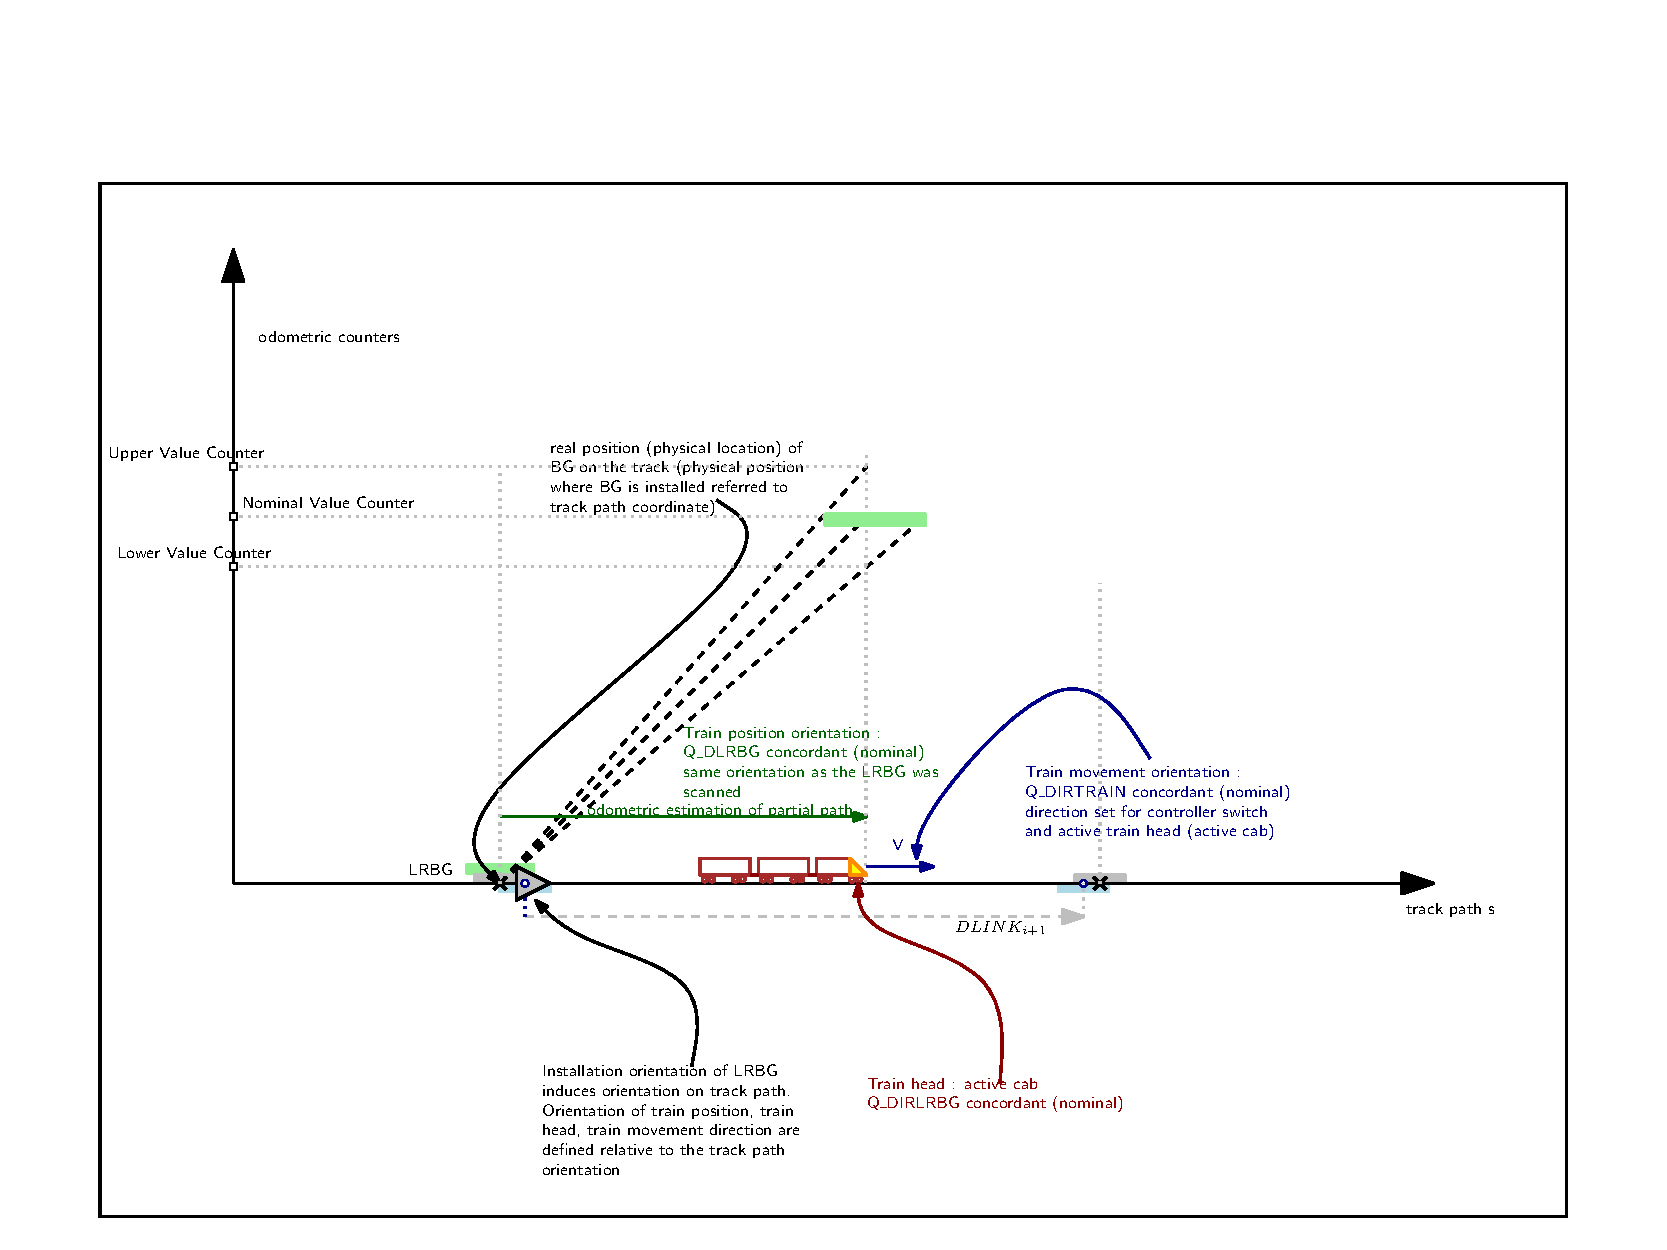
\includegraphics[angle=0,width=0.9\textwidth]{orientation_ontrack_v1.pdf}
}
\caption{\emph{orientation convention}}
\label {fig:orientation}
\end{figure}

The \gls{MMU} is making also movement detection and movement direction detection as reflected by API outputs MOTION\_STATE and MOTION\_DIRECTION. No train movement detection (train standing still) implies also that there will be no train movement direction detection, in such a case the detected train direction is said to be unknown. This outputs will be delayed by the window function needed to stabilize reliable detection. 
The \gls{MMU} orientation establishing the counter behavior is non volatile and non switchable. If in the engine there are two \gls{OBU}s installed then each \gls{OBU} will have it's own wired Cab A irrespective of the configuration adopted for the other \gls{OBU}. The two \gls{OBU}s will never compete for \gls{MMU} data.

When the \gls{OBU} is in a mode referencing to a LRBG, the directions relevant for train driving are given by the following triple (relative to LRBG orientation):
\begin{itemize}
\item Q\_DIRLRBG Train Orientation => active cabin, => Front End => headlights
\item Q\_DIRTRAIN direction of train movement (not the detected motion direction but the direction as set by direction controller switch.
When reversing is allowed this orientation can be reverted operating on the direction switch allowing the train to proceed in reverse direction)  possible values are : nominal (e.g. train oriented nominal and direction switch forward), reverse (e.g. train orientation nominal and direction switch reverse) unknown direction switch in neutral position. The ETCS system will supervise the direction of motion and allow to switch in the reverse direction (opposite to train direction) only under foreseen conditions e.g. during emergency in tunnel.
\item Q\_DLRBG "scanning" orientation at time of over-passing the LRBG and therefore "sign" of the coordinate relative to LRBG (positive coordinate direction means train has scanned LRBG in nominal direction reading increasing N\_PIGs and is now on the arrow tip side of LRBG). The absolute value of this coordinate is given by the variable D\_LRBG.
\end{itemize}
The above three quantities have to be considered as software variables, that need to be initialized and may change depending on the actual state and inputs elaborated. They have only meaning if the direction of the LRBG is given.

other relevant Direction qualifier are :
\begin{itemize}
\item Q\_DIR message orientation (relative to sending BG) nominal (message valid for nominal scanning/overpassing of the BG) reverse and neutral (valid for both directions) In case of RBC sending the message the reference orientation is given by the one of the LRBG.
This direction qualifier is most relevant for giving the relative position of a MA (Packet 12) transmitted by a BG  in respect to relevant train end. This gives the permitted movement direction of the train, and if an opposite movement direction is detected, by evaluating the \gls{MMU} output MOTION\_DIRECTION a brake command should be triggered.
\item Q\_LINKORIENTATION part of a linking vector (packet 5) indicates if the linked BG pointed by the vector will be over-passed in nominal or reverse direction.
\end{itemize}


other Direction qualifier are :
\begin{itemize}
\item Q\_MPOSITION orientation of kilometer counting convention
\item Q\_ORIENTATION orientation given by RBC to a passed LRBG
\end{itemize}

\clearpage

\subsection{Rail-routed path and empirical odometric map}
The estimation of the train position is currently based on the odometric measure of the distance traveled by the train made with an on board equipment and by the detection of reference balises installed at known positions on the track, when the Balise receiver antenna detects them. 
The distance is measured along the rail or track path. Actually track routes can have variable branches (when crossing switch points from blade side). The on-board odometry is not able to map different branches and will only trace an one-dimensional path.

\begin{figure}[!ht]
%\boxed{
\centerline{
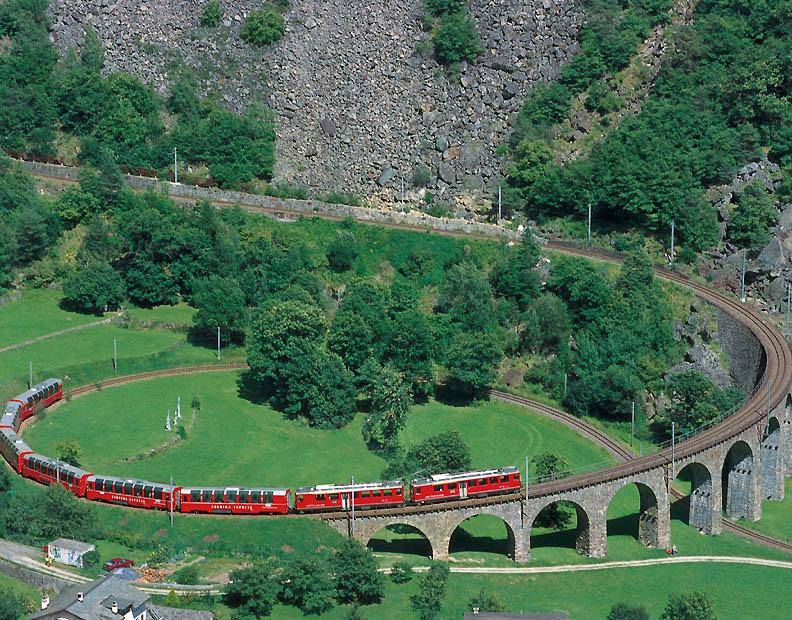
\includegraphics[angle=-0,width=.38\textwidth]{Brusio_RSLB.jpg}
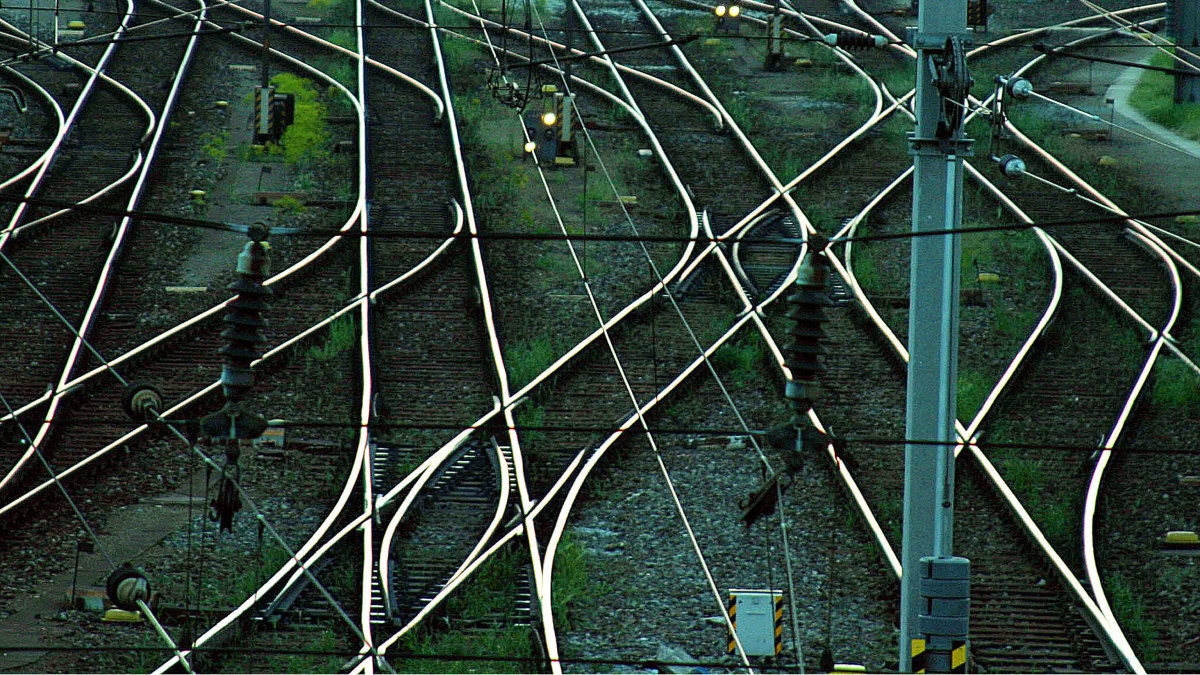
\includegraphics[angle=-0,width=.53\textwidth]{deviate.jpg}
}
%}
\caption{\emph{Examples of train path}}
\label {fig:trainpath}
\end{figure}
The picture in figure \ref{fig:trainpath} gives two illustrative examples of rail path.
Even if the train route can follow different branches depending on the position of the switches the coordinate system available on-board is always one-dimensional and needs to get updated track data for the selected route each time the train passes over a switch point from blade side. 

This is done mainly through the so-called repositioning information\footnote{see \gls{SRS} 026 3.8.5.3.5.} available at a BG immediately after the branch point. Such a balise group is usually announced by a weak link \footnote{3.4.4.2. and 3.4.4.4.} not including the id\footnote{id number 16383 } of the BG and applying a relaxed expectation window.
\begin{figure}[!ht]
\centerline{
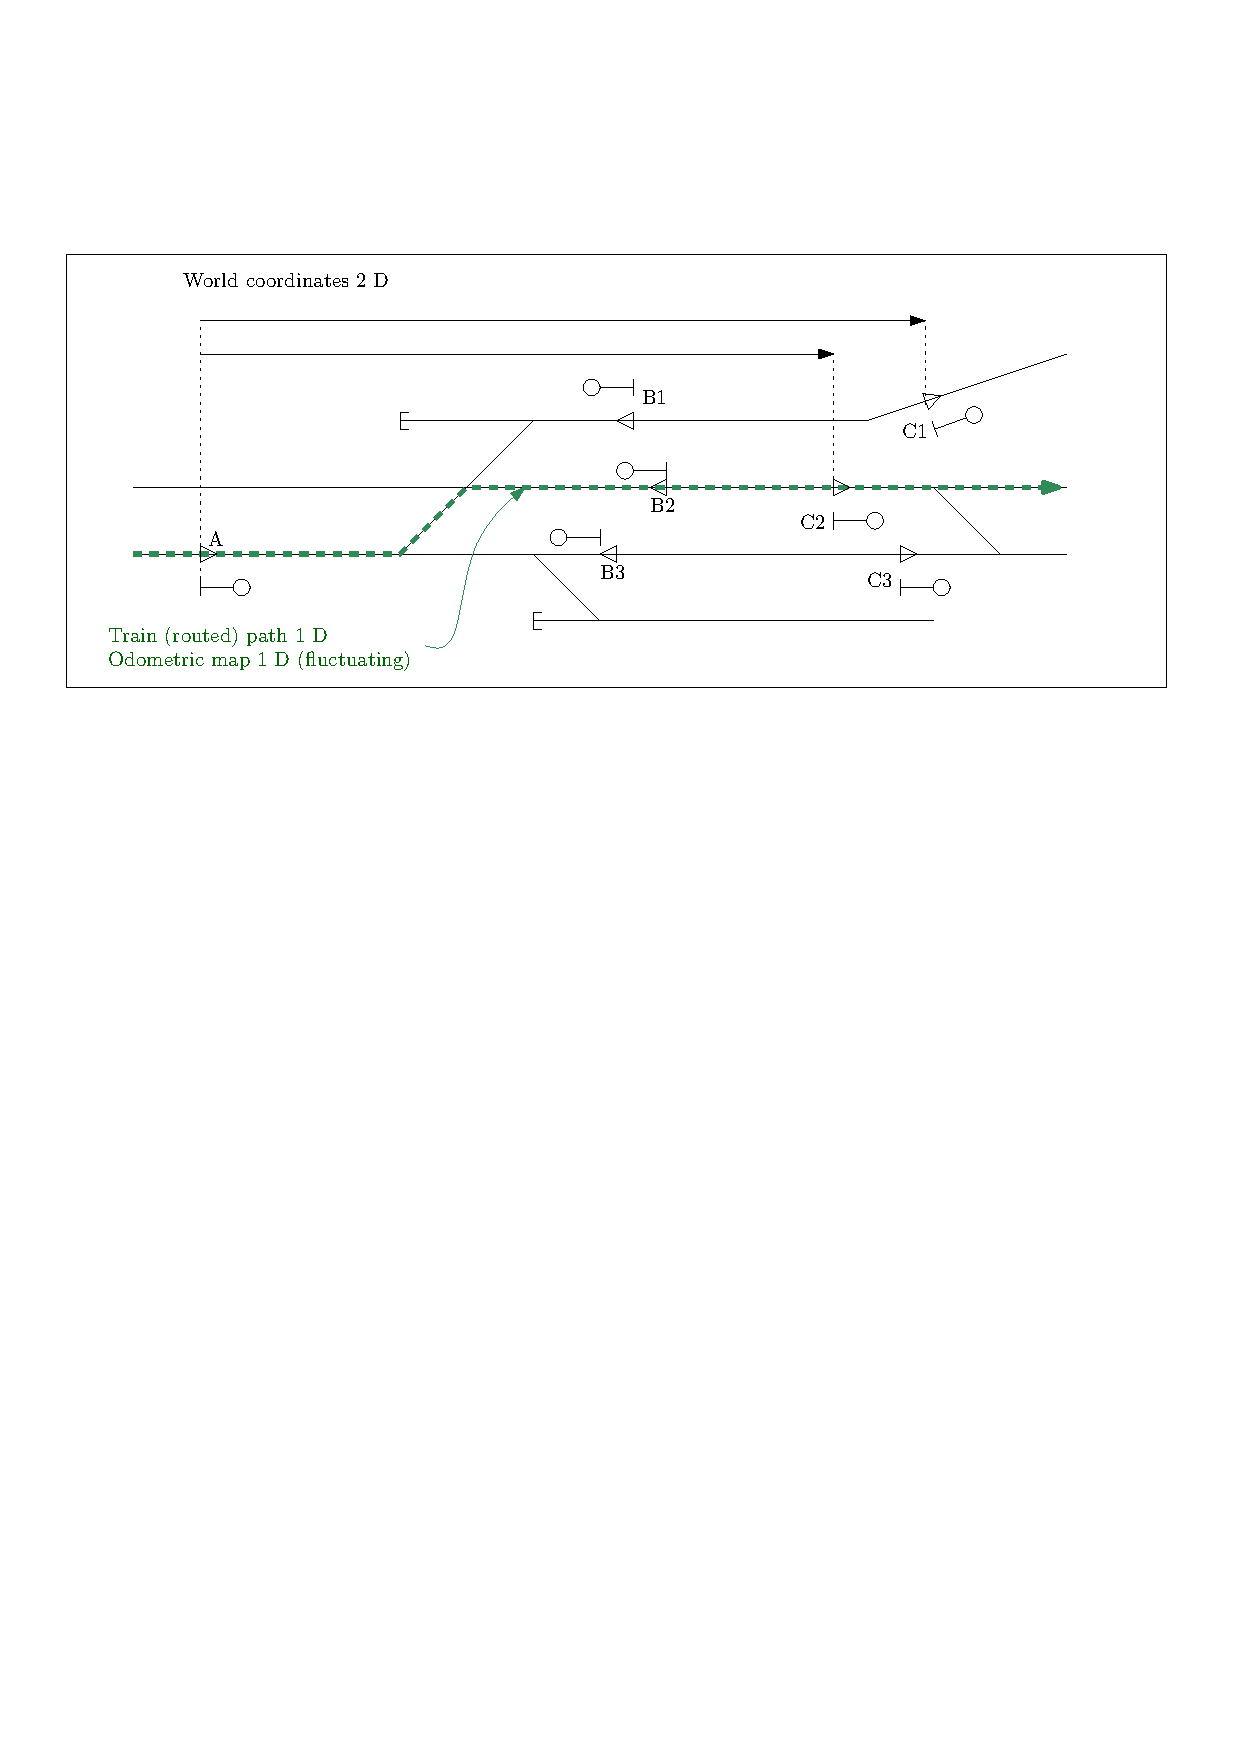
\includegraphics[angle=-0,width=.8\textwidth]{trainroute_v2.pdf}
%\includegraphics[angle=-0,width=.5\textwidth]{fig24_v1.png}
}
\caption{\emph{Example of repositioning data.}}
\label {fig:Fig24}
\end{figure}
Note: In cases where a balise group contains repositioning \footnote{By convention \emph{relocation} indicates a coordinate shift along the the train path, while \emph{repositioning} indicates a displacement in the second dimension, which is not tracked by the on-board equipment} information, the term linked also applies since the balise group is announced, marked as linked and contains repositioning information marked accordingly. For clarity sometimes we will use the term weakly linked. Repositioning information contained in a balise group message shall only be evaluated if linking information has announced a following balise group as unknown but containing repositioning information. A balise group message containing a movement authority shall not contain repositioning information for the same direction.

In the balise group A the following information is given:
\begin{itemize}
\item The most restrictive track description from all routes (which could be a combination
from the routes);
\item The linking distance given to the farthest balise group containing repositioning
information, the identification of the repositioning balise group is not known;
\item For a given aspect of signal A, the most restrictive MA from all routes (the shortest
sections from the routes and the lowest target speed at the End Of Authority);
\item If some sections are time limited, the most restrictive timer.
\end{itemize}
Balise groups B (B 1 or B 2 ) give the following static information (repositioning information):
\begin{itemize}
\item Linking to the next balise group C
\item The distance to the end of the current section (i.e. the distance to the end of section
B1 - C1, or the distance to the end of section B2 - C2)
\item The track description related to this track.

\end{itemize}

\subsubsection{Mitigation of balise cross-talk while expecting repositioning information}
If repositioning is announced and the expected repositioning balise group has been found, the ERTMS/ETCS on-board equipment shall keep looking for a balise group that satisfies the same criteria as this previously expected and already found
repositioning balise group, until one of the following events occurs:
\begin{itemize}
\item the on-board antenna leaves the expectation window of the repositioning balise group that was announced and already found
\item a linked balise group that has been announced with known identity is found.
\end{itemize}
If a second balise group is found that satisfies the same criteria as the previously
expected and already found repositioning balise group, the ERTMS/ETCS on-board
equipment shall command the service brake and the driver shall be informed. At
standstill, the location based information stored on-board shall be shortened to the
current position. Refer to appendix Subset 026 A.3.4 for the exhaustive list of information, which shall be shortened.

Note: this function is independent from linking function, i.e. the rules related to
linking always apply. This means that once a repositioning balise group has been found and if this latter contains new linking information, the ERTMS/ETCS on-board equipment will start expecting the first balise group announced in this new linking information in parallel with the monitoring specified for mitigating balise reception degradation


\subsection{Correlating two linked BG detections}
%\begin{figure}[!ht]
%\centerline{
%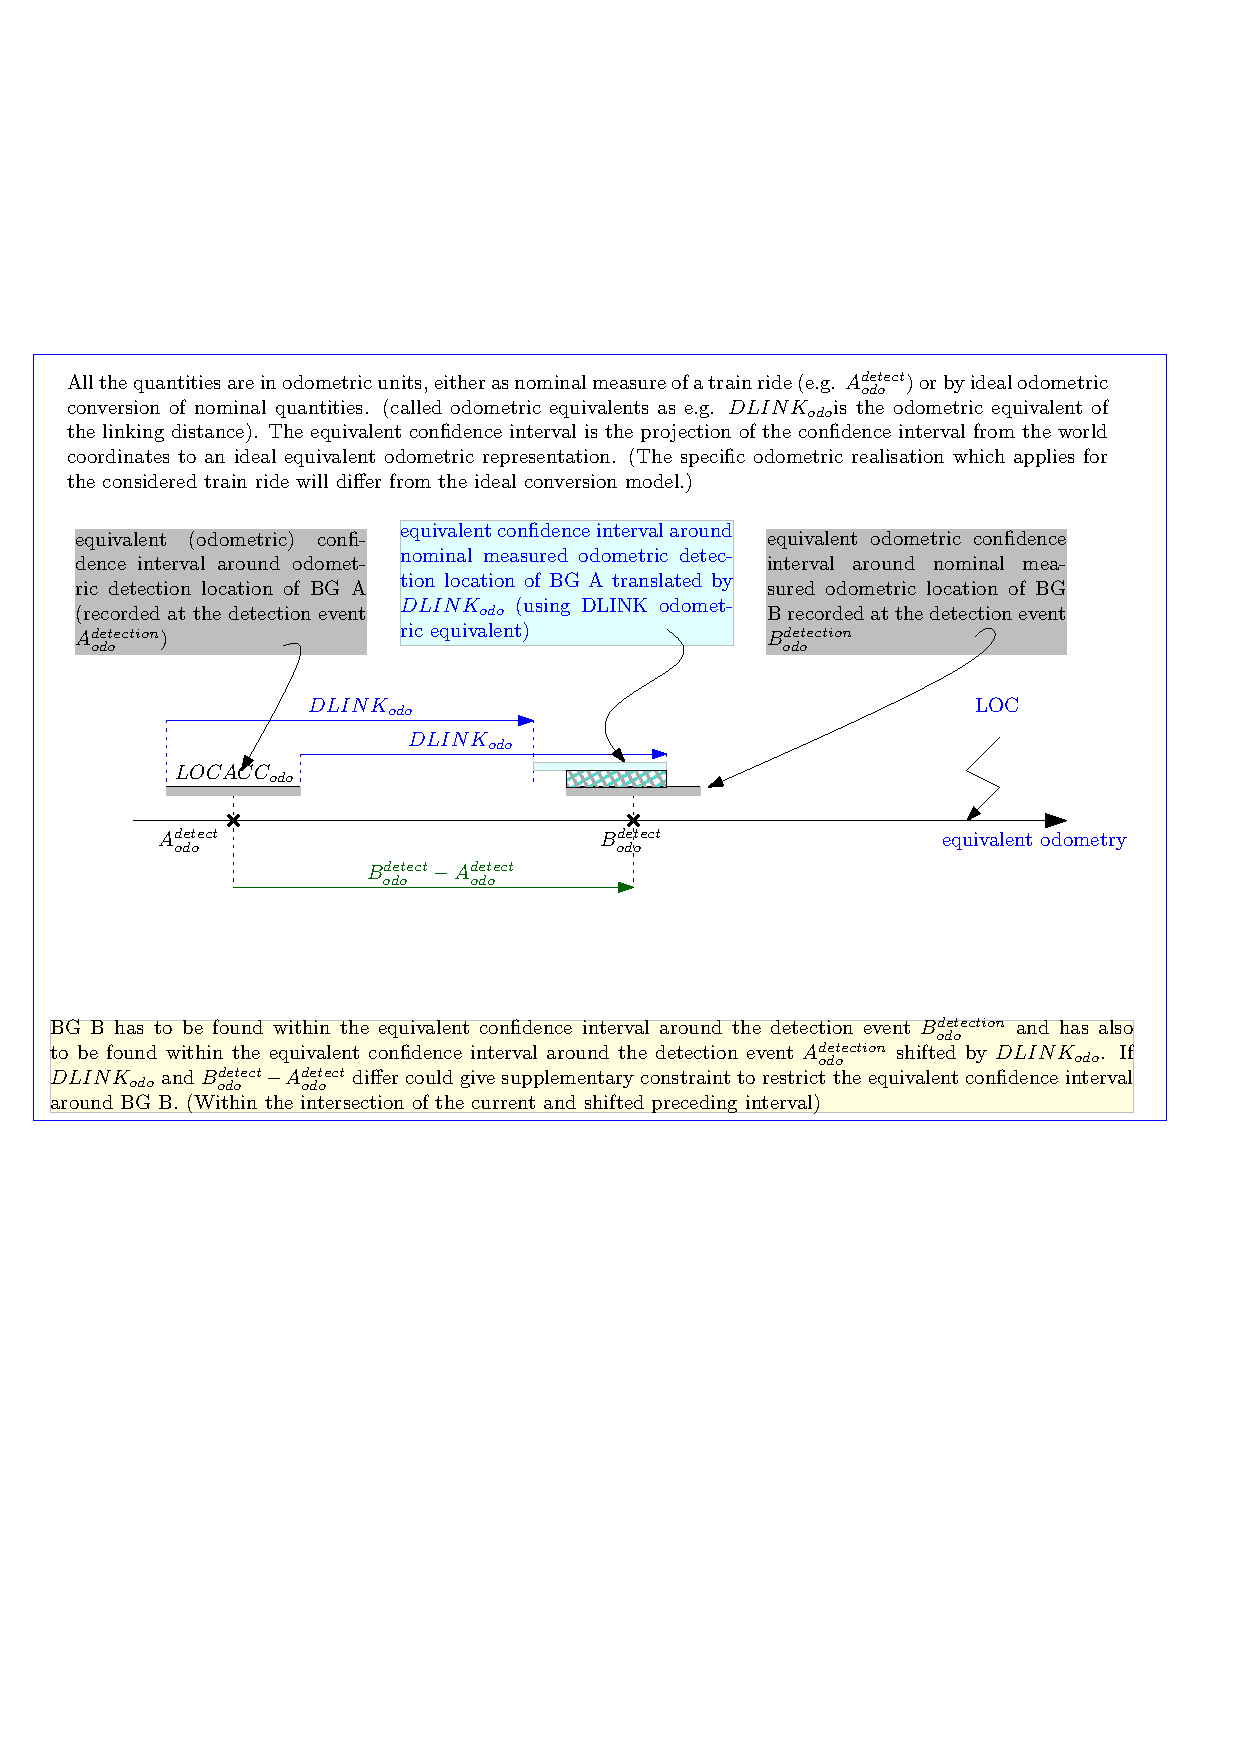
\includegraphics[angle=0,width=.9\textwidth]{odomap_v1.pdf}
%}
%\caption{\emph{Supplementary information}}
%\label {fig:odomap}
%\end{figure}
If the odometric difference between two linked BG detections differs from nominal distance in a significant way (at least more than the odometric error of 5 \% in plus or in minus) this supplemental information can be used to constrain the reciprocal confidence interval of the second detected BG.


\subsection{Odometry from Wheel motion}

In the following we try to adopt an uniform symbol convention, based on the assumption that there are quantities measured at fixed time intervals and quantities measured at variable, speed dependent time intervals. Fixed time intervals are :
\begin{equation}
\tau^\star =1\, \mu s ,\,
\tau^\circ = 50 \,ms, \,
\tau^\bullet = N^\bullet \tau^\circ = 500\, ms
\end{equation}
Variable time intervals are given by the time between the detection of two odometer teeth or two odometer virtual teeth.

\begin{figure}[!ht]
\centerline{
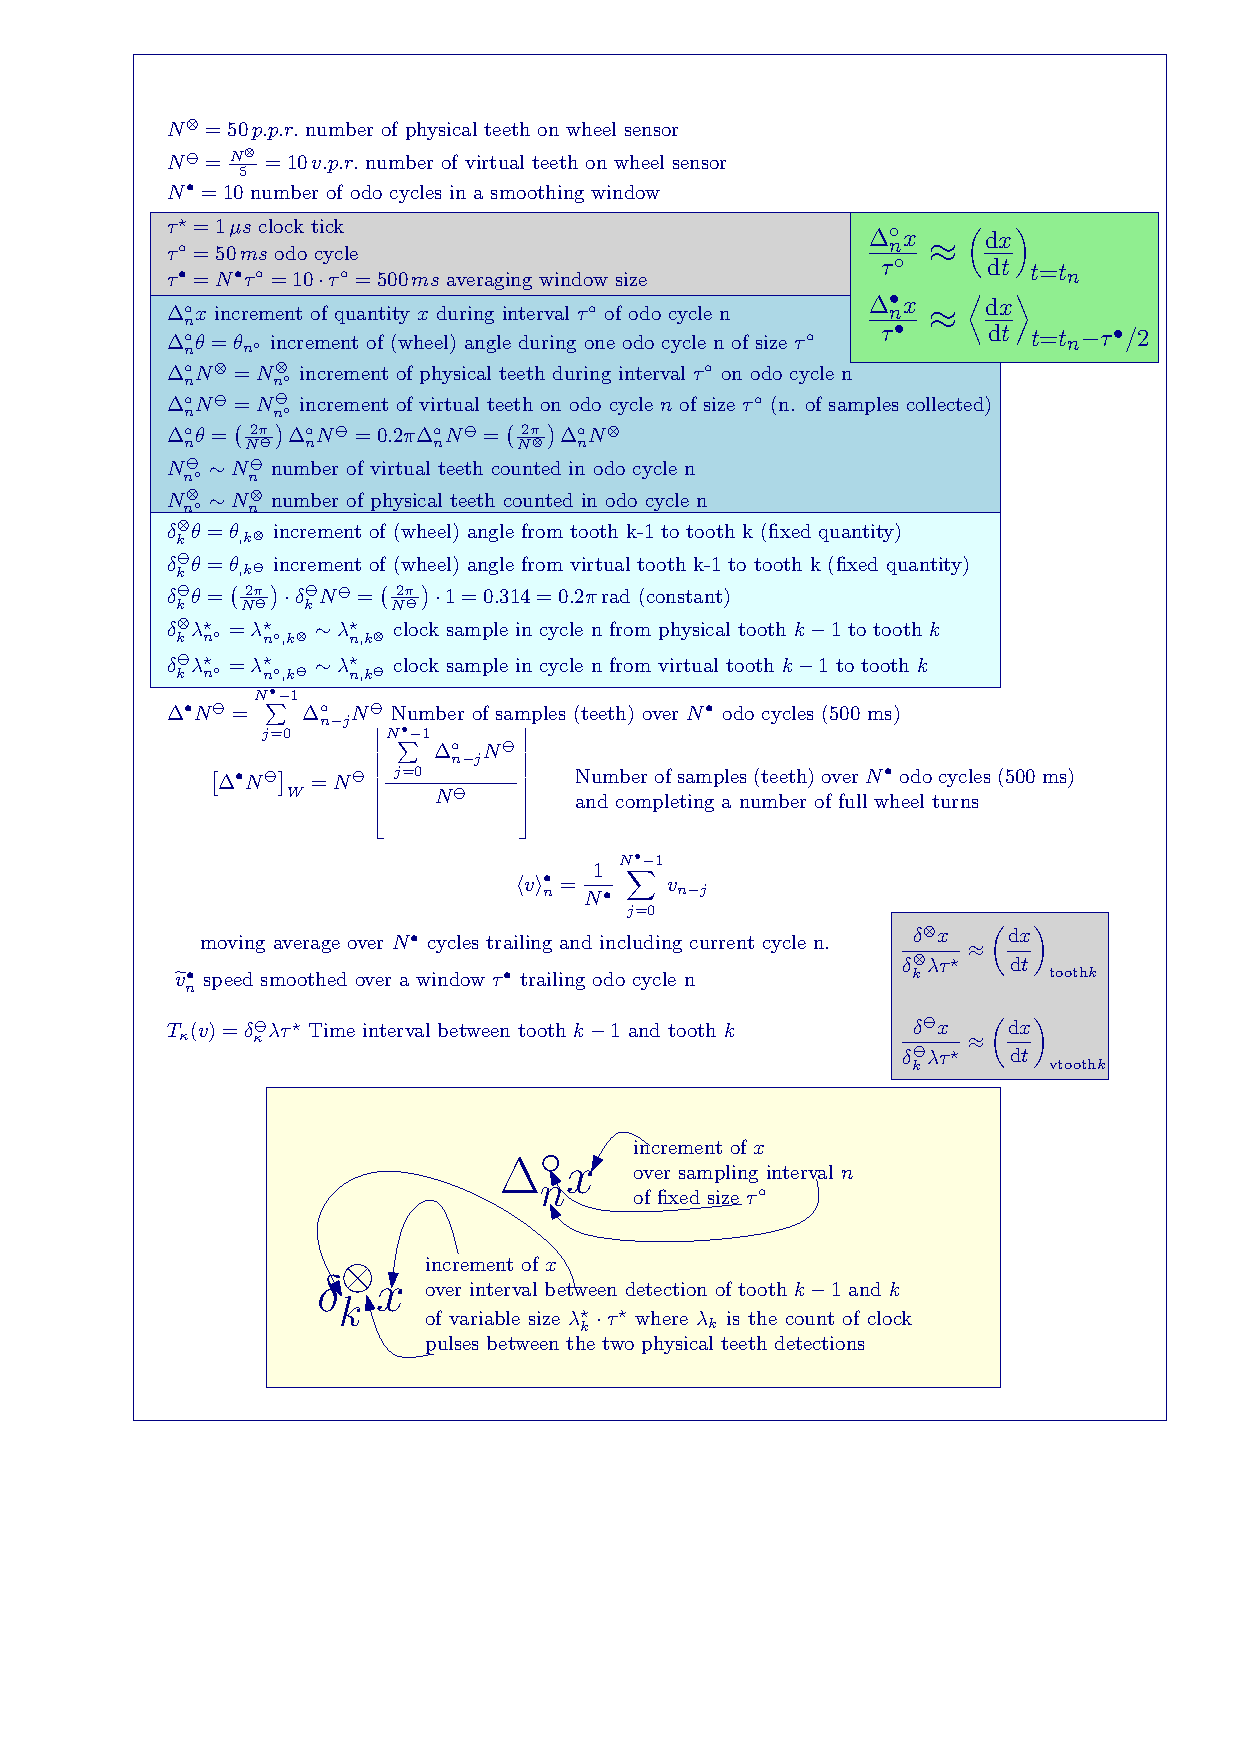
\includegraphics[angle=0,width=.95\textwidth]{symbols_used_v2.pdf}
}
\caption{\emph{explanation to symbols used in following text}}
\label {fig:symbolu}
\end{figure}
\begin{figure}[!ht]
\centerline{
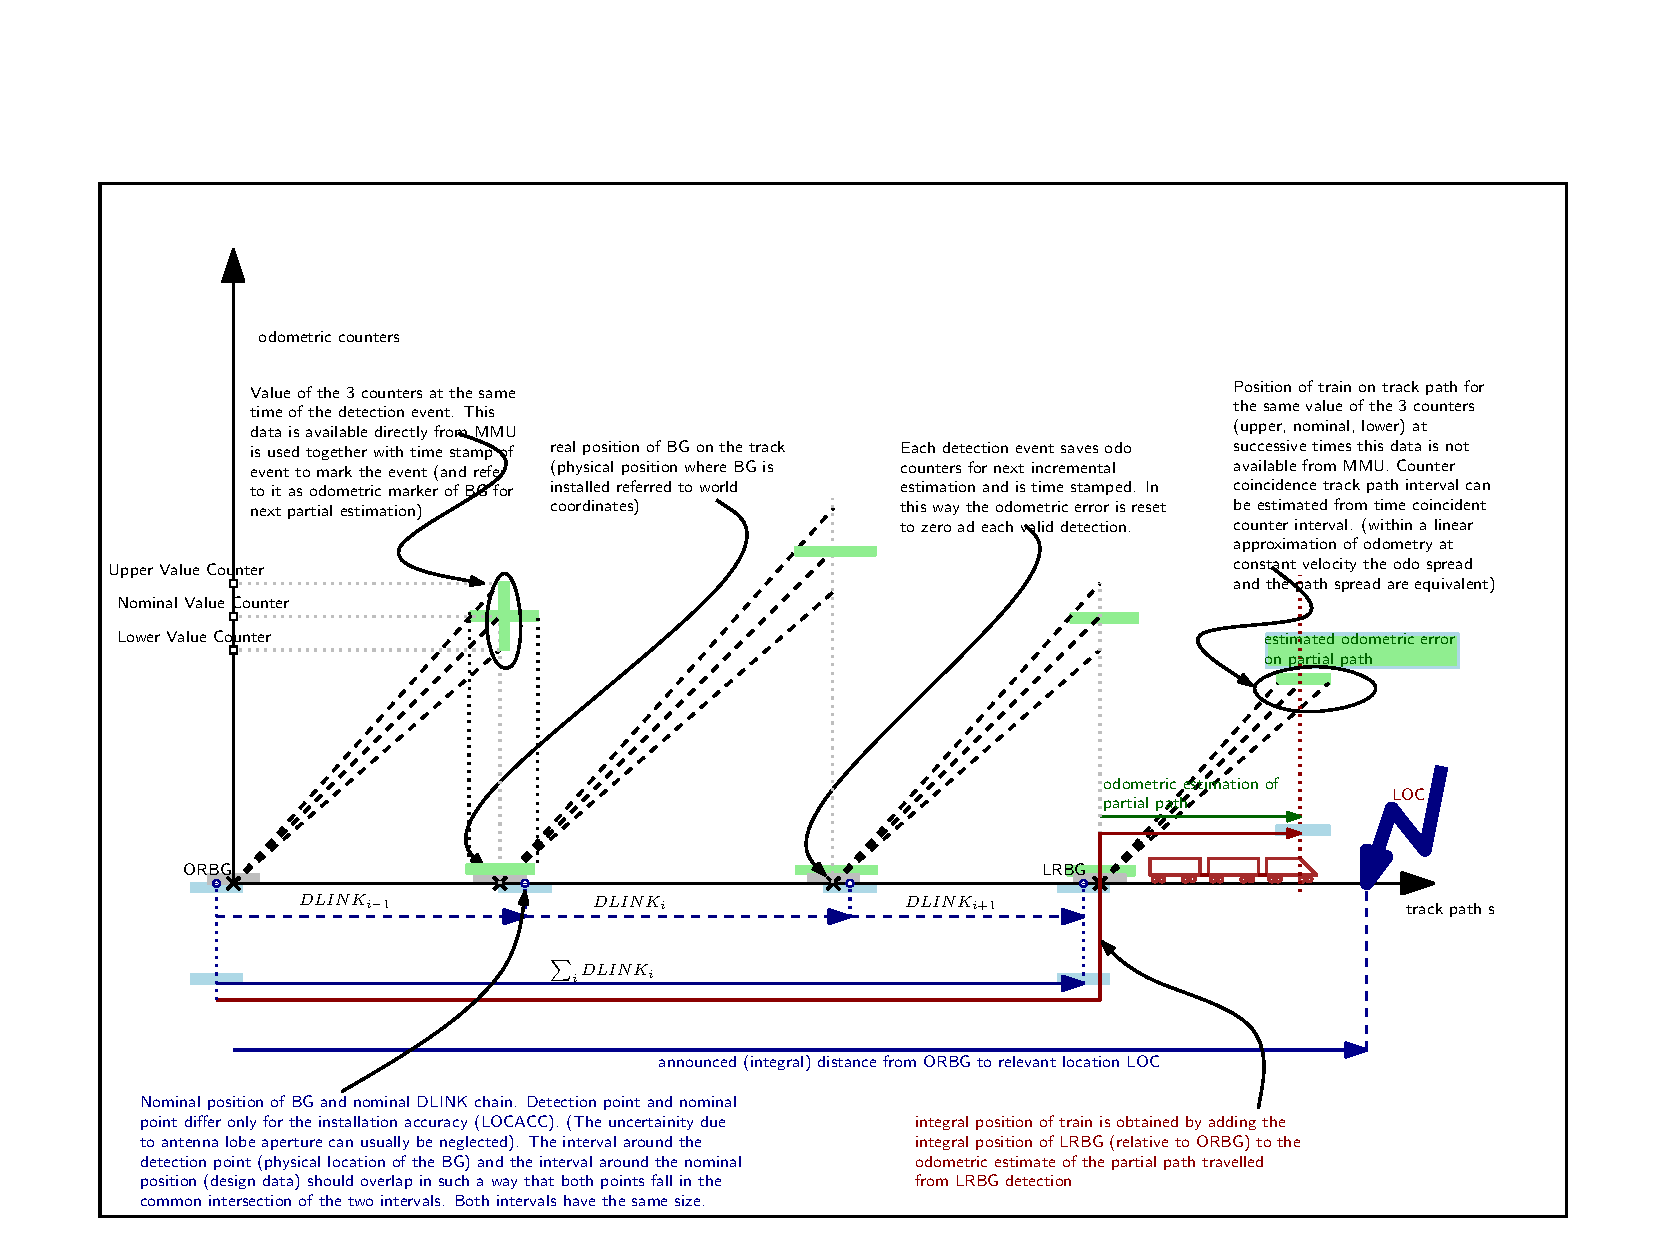
\includegraphics[angle=0,width=1.\textwidth]{odo_linear_II.pdf}
}
\caption{\emph{odometric conversion}}
\label {fig:odoconv}
\end{figure}
\subsubsection{Basic principles for odometry modeling}
The main role/function of the \gls{MMU}  involves acquiring the measured physical quantities on the various sensors, to process
them and to supply, in safety, to each EVC main unit the following set of information:
\begin{itemize}
\item A speed range [speed min , speed nom , speed max ].
\item A cumulated distance range [distance min , distance nom , distance max ].
\item An acceleration range [acceleration min , acceleration nom , acceleration max ].
\item The direction of travel (\gls{DOT}).
\item The motion information.
\item The adhesion loss detection.
\end{itemize}
\newpage
\subsubsection{Odometry model performance}

\begin{tabular}{|l| l|}
\hline
Measure / Estimate  & examples of range / value for an odometry model\\
\hline
Distance accuracy & $\pm$(4m + 5\%) \\
\hline
Speed accuracy & $\pm$ 2 km/h for v$<$ 30 km/h, \\ 
&then increasing linearly up to $\pm$ 12 km/h at v = 500 km/h \\
\hline
%\colorbox{yellow}
{Speed \emph{resolution}} 
%(DESG 0648\_105) 
& $\frac{2\pi R}{N^\ominus\cdot \tau^\circ } = \frac{0.314 m}{.05 s}\,  (\approx 6.28\, m/s \approx 22.6\, km/h)$ \\ & minimal speed to have at least one new sample each cycle\\
\hline
data acquisition cycle $\tau^\circ$ &  50 ms between measurement \\
\hline
Cycle time  & Data transmission to Core each 100 ms\\
\hline
Distance resolution & 0.34 m (min for standstill detection = 0.5 m)\\
\hline
Speed resolution (GATC DESG 0638) & 0,025 m/s $(\approx 0.1\, \mathrm{km/h} )$ \\
\hline
Speed range & 0 to 500 km/h \\
\hline
Direction of travel (\gls{DOT}) &Mandatory in objective SIL4\\
\hline
 Motion detection & Motion detected if v $>$ 0,5 km/h max or d $>$ 0,5 m max \\
\hline
 Safety Integrity Level & SIL4\\
\hline

\end{tabular}

\subsubsection{Encoders and \gls{WS}}

Incremental encoders provide a specific number of equally spaced pulses per revolution (PPR) or per inch or millimeter of linear motion. A single channel output is used for applications where sensing the direction of movement is not important. 
\begin{figure}[ht!]
\centerline{
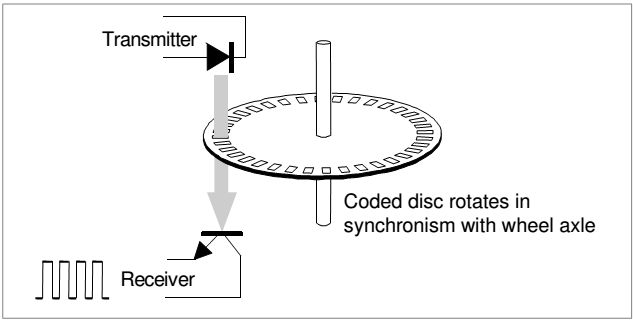
\includegraphics[angle=0,width=.5\textwidth]{impulsweggeber.jpg}
}
\caption{\emph{wheel sensor}}
\label {fig:wsens}
\end{figure}
Where direction sensing is required, quadrature output is used, with two channels 90 electrical degrees out of phase; circuitry determines direction of movement based on the phase relationship between them. This is useful for processes that can reverse, or must maintain net position when standing still or mechanically oscillating. For example, machine vibration while stopped could cause a unidirectional encoder to produce a stream of pulses that would be erroneously counted as motion. The controller would not be fooled when quadrature counting is used.

When more resolution is needed, it is possible for the counter to count the leading and trailing edges of the pulse train from one channel, which doubles (x2) the number of pulses counted for one rotation or inch of motion. Counting both leading and trailing edges of both channels will give 4x resolution.
\begin{figure}[ht!]
\centerline{
%\includegraphics[angle=0,width=.35\textwidth]{counting.png}
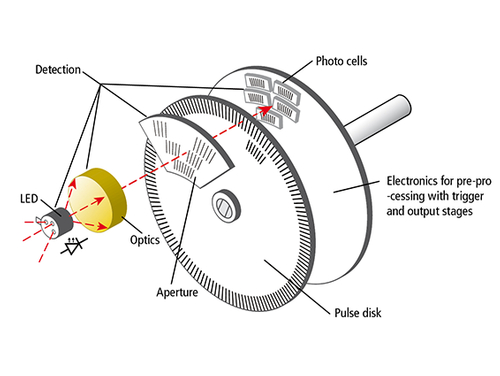
\includegraphics[angle=0,width=.35\textwidth]{increm_det_en.png}
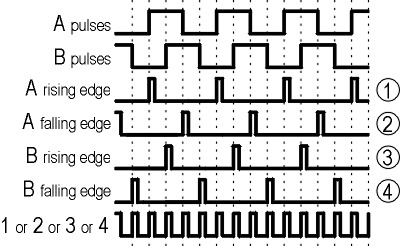
\includegraphics[angle=0,width=.35\textwidth]{quad.jpg}
}
\caption{\emph{encoder output}}
\label {fig:ienc}
\end{figure}
An incremental encoder’s output indicates motion. To determine position, its pulses must be accumulated by a counter. The count is subject to loss during a power
interruption or corruption by electrical transients. When starting up, the equipment must be driven to a reference or home position to initialize the position counters. Some incremental encoders also produce another signal known as the “marker,” “index,” or “Z channel.” This signal, produced once per revolution of a shaft
encoder or at precisely-known points on a linear scale, is often used to locate a specific position, especially during a homing sequence.
Resolution is the number of measuring segments or units in one revolution of an encoder shaft or one inch or mm of a linear scale. Shaft encoders are available with
resolutions up to 10,000 pulses per revolution (PPR) directly, and 40,000 PPR by edge-detection of the A and B channels, while linear encoders are available with
resolutions measured in microns. 
The bottom line is, the selected encoder must have resolution equal to or better than that required by the application. But resolution is not the whole story. Accuracy and resolution are different, and it is possible to have one without the other. This figure shows a distance X divided into 24 increments or “bits.” If X represents $360\deg$ of shaft rotation, then one revolution has been resolved into 24 parts.
\begin{figure}[ht!]
\centering
\begin{tabular}{c}
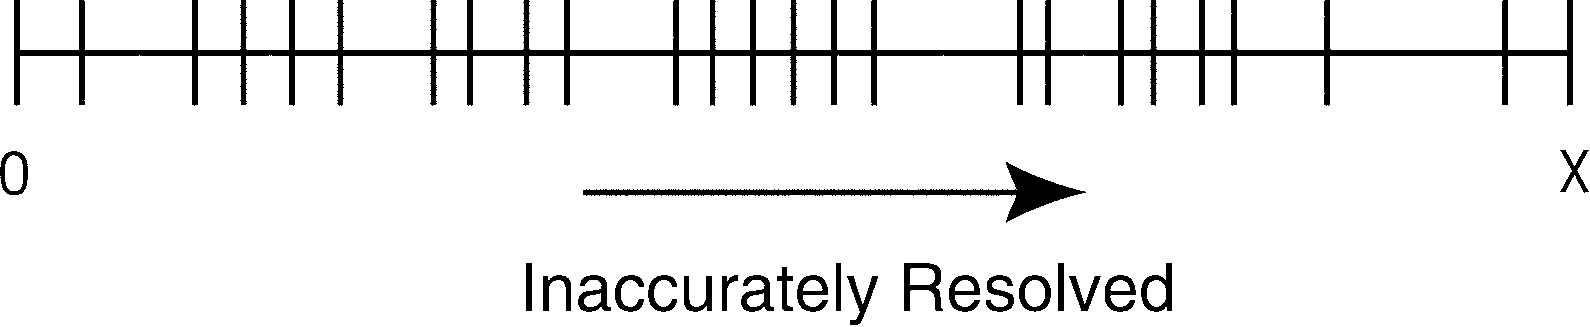
\includegraphics[angle=0,width=.5\textwidth]{accuracy.png} \\
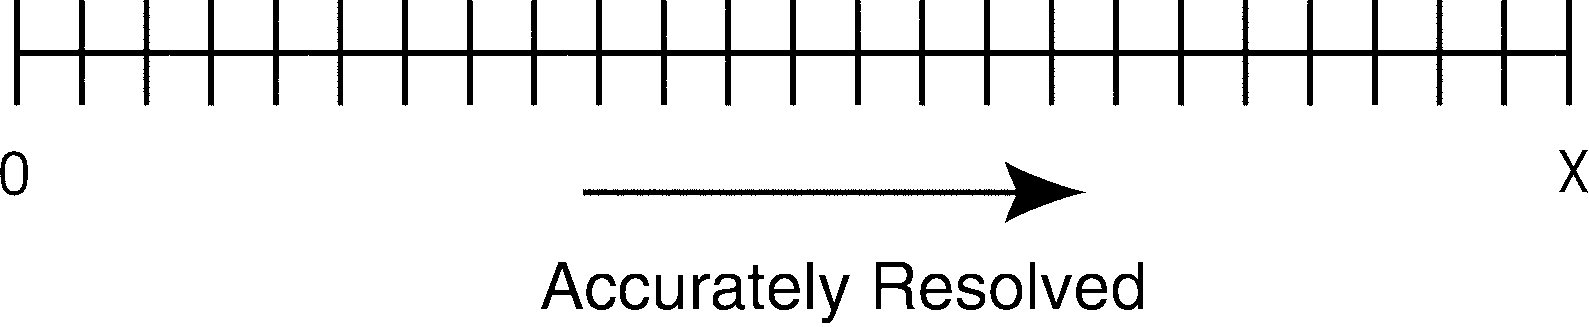
\includegraphics[angle=0,width=.5\textwidth]{accuracy2.png}
\end{tabular}
\caption{\emph{accuracy}}
\label {fig:encaccu}
\end{figure}
While there are 24 bits of resolution, the 24 parts are not uniform. This transducer could not be used to measure position, velocity or acceleration with any accuracy. On the other hand, in this figure the distance X is divided into 24 equal parts. Each increment represents exactly 1/24 of a revolution. This transducer operates with accuracy as well as resolution. Accuracy, however, can be independent of resolution. A transducer may have a resolution of only two parts per revolution, yet its accuracy could be $\pm 6$ arc seconds.

System Accuracy: An encoder performance is typically stated as resolution, rather than accuracy of measurement. The encoder may be able to resolve movement into precise bits very accurately, but the accuracy of each bit is limited by the quality of the machine motion being monitored. For example, if there are deflections of machine elements under load, or if there is a drive screw with 0.1 inch of play, using a 1000 count-per-turn encoder with an output reading to 0.001 inch will not improve the 0.1 inch tolerance on the measurement. The encoder only reports
position; it cannot improve on the basic accuracy of the shaft motion from which the position is sensed.

System Repeatability: Repeatability is the tolerance to which the controlled machine element can be repeatedly positioned to the same point in its travel. Repeatability is generally less than system resolution, but somewhat better than system accuracy. 10,000 pulses per turn can be generated from a 2500 cycle, two channel encoder. Typically with a Dynapar encoder, this 4x signal will be accurate to better than $\pm 1$ count.

Resolution is the ability to 'resolve' differences; that is, to draw a distinction between two things. High resolution means being able to resolve small differences. In a digital system, resolution means the smallest increment or step that can be taken or seen. In an analog system, it means the smallest step or difference that can be reliably observed. 

The accuracy of a system refers to how much the system, whether in measurement or control, deviates from the truth. To be meaningful, accuracy must really refer to 'worst case accuracy'.
As a trivial example, a stopped, unworking clock is still correct twice a day! We must describe this unworking clock by its worst case accuracy, which would be +/- 6 hours. Sometimes the '+/-' is dropped and the extent of the inaccuracy is reported: for this clock, it would be 12 hours.
Beyond describing the worst case, we must also consider resolution. The following is very important:
The accuracy of a system can never exceed its resolution! This follows from the worst case requirement.

Repeatability is the variance in repeated measurements on an unchanging sample. If measured statistically, it is sometimes referred to as the noise level in the measurement. In general, high repeatability means a low noise level. Precision is used in different ways depending on context.
By design, measurement resolution is normally set better than accuracy. In the case of contact angle measurements, the resolution might be 0.01 degree but the absolute accuracy 1 degree. Why have resolution better than accuracy? One reason is that often accuracy is limited by the availability of calibration standards to show or prove the accuracy. If the best available standard is +/- 0.5 degrees, you can not claim an accuracy better than that. However, the ability to measure small differences between samples, whatever the absolute number, is useful and for this reason a higher resolution is provided. In general, instruments can measure repeatedly the same sample with a variance of a few units of resolution. This is called the noise level of the measurement. If we report a resolution of 0.01 degree, we expect to measure a static sample with a repeatability of, say, +/-0.02 or 0.03 degrees. 

\subsection{Speed measure}
The\footnote{Petrella Speed Measurement Algorithms for Low-Resolution Incremental Encoder Equipped Drives: a Comparative Analysis \cite{petrella}} classical and probably the simplest method to measure rotor speed is the direct measure of the frequency of the encoder pulses. 

\begin{figure}[ht!]
\centerline{
%\includegraphics[angle=0,width=.35\textwidth]{counting.png}
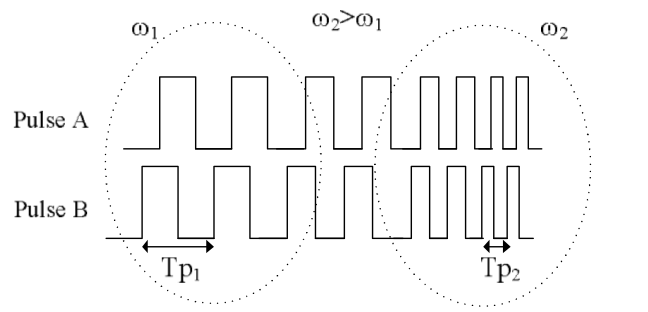
\includegraphics[angle=0,width=.5\textwidth]{speed_var.png}
}
\caption{\emph{encoder output while speed increases}}
\label {fig:v-var}
\end{figure}
Typically the number of the observed pulses inside a given and constant-width time-window is counted. Angular speed is then approximated to the discrete incremental ratio, that is constant speed is considered inside the observation windows:
\begin{equation}
\omega=\frac{\mathrm{d}\theta}{\mathrm{d}t}\approx\frac{\Delta_{n}^\circ\theta}{\tau^\circ}=\left(\frac{2\pi}{N^\otimes }\right) \frac{\Delta_n^\circ N^\otimes}{\tau^\circ}
\end{equation}

Where $N^\otimes$ is the number of pulses per revolution, $\Delta^\circ_n \theta$ is the angular increment and $\Delta^\circ_n N$ the corresponding number of pulses counted within the cycle n corresponding (observation window of fixed size $\tau^\circ$).  As a concrete model we assume to have following values $ N^\otimes = 50 \,\mathrm{p.p.r.} $ (pulses per revolution) a wheel diameter of about $ R \approx 1\, \mathrm{m}$ (ICE trains have about 980 mm, while Euro-sprinter are between 1.1 and 1.2m) at $\varv_{train} = 5 \mathrm{km/h}=1.4 \,\mathrm{m/s}$
whith $\tau^\circ=50 \, m\mathrm{s}$ we get:
\begin{equation}
\boxed{
\Delta_n^\circ N^{\otimes}= \varv_{train}[m/s]\cdot \left(\frac{\tau^\circ}{2\pi R}\right)\cdot N^\otimes=1.4\cdot\frac{0.05}{3.14}\cdot 50 = 1.4\cdot \left(0.796\right) =1.1 }
\end{equation}

We observe that at low speeds there will be no increment in pulse counter $\Delta^\circ_n N^\otimes$ within the observation window $\tau^\circ$ (no variation is detected in one single \gls{MMU} cycle, the counter may vary after more than one \gls{MMU} cycle).
%$\mathfrak{N} \!\!\!\!\backslash $  $ \check{N} N^{\bullet}$

\begin{tabular}{|l|l | l| l|}
\hline
speed $\varv$ [km/h] &speed $\varv$ [m/s]&  approximate pulse (teeth) count & virtual teeth \\ &  & in a $50\,\mathrm{m}s $ time window ($\varv \cdot 0.796$) & $\Delta_n^\circ N/5$\\
\hline
$\varv_{train}\approx 1\, \mathrm{km/h}$ & 0.28 m/s & $\Delta_n^\circ N^\otimes\approx 0.22 $ & $\Delta_n^\circ N^\ominus \approx  .044 $ \\
\hline
$\varv_{train}\approx 3.6\, \mathrm{km/h}$ & 1 m/s & $\Delta_n^\circ N^\otimes\approx 0.796 $ & $\Delta_n^\circ N^\ominus \approx  .159 $\\
\hline
$\varv_{train}\approx 5\, \mathrm{km/h}$ & 1.4 m/s & $\Delta_n^\circ N^\otimes\approx 1.1 $ & $\Delta_n^\circ N^\ominus \approx  .22 $ \\
\hline
$\varv_{train}\approx 10\, \mathrm{km/h}$ & 2.8 m/s & $\Delta_n^\circ N^\otimes\approx 2.2 $ & $\Delta_n^\circ N^\ominus \approx  .44 $ \\
\hline
$\varv_{train}\approx 11.3\, \mathrm{km/h}$ & 3.14 m/s & $\Delta_n^\circ N^\otimes\approx 2.5 $ & $\Delta_n^\circ N^\ominus \approx  .5$ \\
\hline
%\colorbox{yellow}
{$\varv_{train}\approx 22.6 \,\mathrm{km/h}$} & 6,28 m/s &
%\colorbox{yellow}
{ $\Delta_n^\circ N^\otimes\approx 5 $} & $\Delta_n^\circ N^\ominus \approx  1 $\\
\hline
$\varv_{train}\approx 36\, \mathrm{km/h}$ & 10 m/s & $\Delta_n^\circ N^\otimes\approx 7.96 $ & $\Delta_n^\circ N^\ominus \approx  1.59 $\\
\hline
$\varv_{train}\approx 50\, \mathrm{km/h}$ & 14 m/s & $\Delta_n^\circ N^\otimes\approx 11 $ & $\Delta_n^\circ N^\ominus \approx  2.2$ \\
\hline
$\varv_{train}\approx 72 \,\mathrm{km/h}$ & 20 m/s & $\Delta_n^\circ N^\otimes\approx 15.92 $ & $\Delta_n^\circ N^\ominus \approx  3.18$\\
\hline
$\varv_{train}\approx 100 \,\mathrm{km/h}$ & 28 m/s & $\Delta_n^\circ N^\otimes\approx 22 $ & $\Delta_n^\circ N^\ominus \approx  4.4 $\\
\hline  
$\varv_{train} \approx 150\, \mathrm{km/h}$ & 42 m/s & $\Delta_n^\circ N^\otimes\approx 33 $ & $\Delta_n^\circ N^\ominus \approx  6.6 $\\
\hline
$\varv_{train}\approx 160 \,\mathrm{km/h}$ & 44.8 m/s & $\Delta_n^\circ N^\otimes\approx 35.66 $ & $\Delta_n^\circ N^\ominus \approx  7.132$ \\
\hline
$\varv_{train}\approx 300\, \mathrm{km/h}$ & 84 m/s & $\Delta_n^\circ N^\otimes\approx 66.864 $ & $\Delta_n^\circ N^\ominus \approx  13.372 $\\
\hline
$\varv_{train}\approx 360\, \mathrm{km/h}$ & 100 m/s & $\Delta_n^\circ N^\otimes\approx 79.6 $ & $\Delta_n^\circ N^\ominus \approx  15.92 $\\
\hline
\end{tabular}

\begin{figure}[ht!]
\centerline{
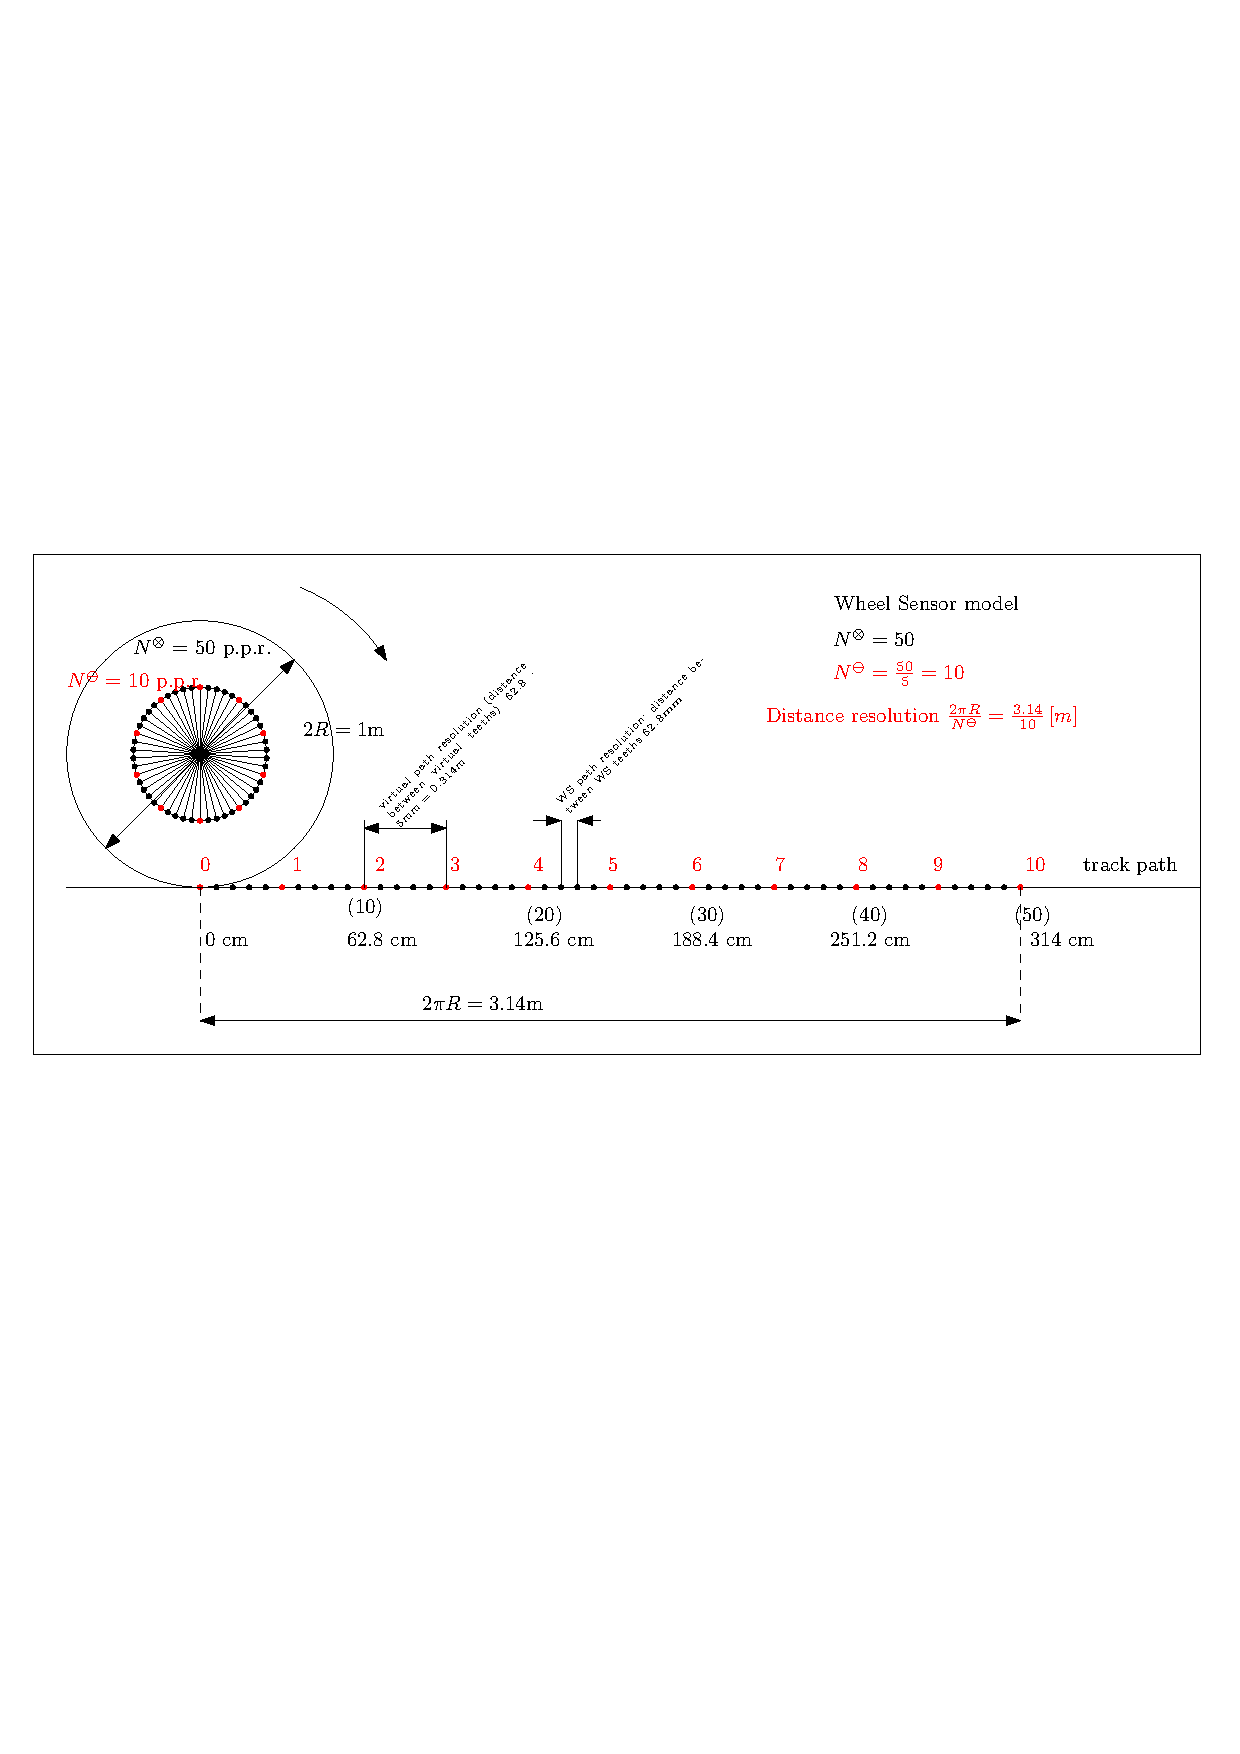
\includegraphics[angle=0,width=.9\textwidth]{virtual_teeths_v3.pdf}
}
\caption{\emph{virtual teeth and path resolution}}
\label {fig:virtualteeth}
\end{figure}
An alternative solution to improve the measurement performance at lower speed is to switch from frequency to period measurement e.g. below a certain level of (low) speed. The measurement is realized by counting the number of periods of a high frequency signal inside one (or more) encoder pulses, Fig. \ref{fig:periodenc}. The following formula is obtained under the hypothesis that motor speed is constant and only one period $\delta^\ominus_k N^\ominus = 1$ of the encoder signal is considered:
\begin{equation}
\omega=\frac{\mathrm{d}\theta}{\mathrm{d}t}\approx \frac{\delta^\ominus_k\theta}{\delta^\ominus_k\lambda^\star\cdot\tau^\star}= \left(\frac{2\pi}{N^\ominus}\right)\frac{1}{\lambda^\star_{,k^\ominus}\cdot\tau^\star}
\end{equation}

A speed sample $\lambda_k$ can be accumulated each period of the encoder signals. The speed sampling period is thus a function of wheel speed:
\begin{equation}
T^\ominus_k(\omega) =\delta^\ominus_k\lambda^\star\cdot\tau^\star = \left( \frac{2\pi}{N^\ominus}\right)  \frac{1}{\omega}=\frac{T_{\gls{WS}}(\omega)}{N^\ominus}
\end{equation}
where $\omega$ is the angular speed of the wheel and $T_{\gls{WS}}$ would be the period of a complete revolution of the wheel sensor at constant angular speed.
The accuracy of the measurement is related to the ratio between the period of the high frequency counter and that of the encoder signals, that is not an integer value as it depends on motor speed. A calculation of absolute and percentage errors is extremely difficult as it involves non-linear rounding functions.
A worst-case condition error could be calculated instead by considering the absolute error of one high frequency pulse, leading to a maximum percentage error limiting locus given by the following formula, i.e. roughly linear with speed:
\begin{equation}
e_k(\omega)=\frac{\tau^\star}{\frac{2\pi}{N^\otimes\cdot\omega}-\tau^\star} = \frac{\omega N^\ominus \tau^\star}{2\pi \left(1-N^\ominus\cdot\frac{\tau^\star}{T_{\gls{WS}}}\right)} \approx \frac{\omega\cdot N^\ominus\cdot \tau^\star}{2\pi}=\frac{N^\ominus\tau^\star}{T_{\gls{WS}}(\omega)} = \frac{\tau^\star}{T^\ominus_k(\omega)}
\end{equation}

(the factor $100$ is omitted)

At very low speed the number of high frequency pulses can be extremely high and %\colorbox{yellow}
{saturation} of the digital timer
employed for measurement can occur. Also a speed sample is not available each speed control period, needing an adaptation of the control parameters. In that situation, the quadrature decoding of the encoder pulses can be exploited in order to reduce the width of the measuring window by a factor of four or a reduction of the frequency of the timer can be considered.

The former solution allows to reduce the speed sampling period and improve the control performance of the drive, but makes the measuring system more sensitive to sensor
nonidealities, including variations in the transition locations
from their nominal values and phasing errors between encoder
channels. When low-cost and low-resolution sensors are
employed, nonidealities play the major role in the
determination of period measuring errors and has to be
carefully analyzed in drive design phase. The latter solution
needs to switch on-line the frequency of the timer and adapt the
coefficients of the equations above.
\begin{figure}[ht!]
\centerline{
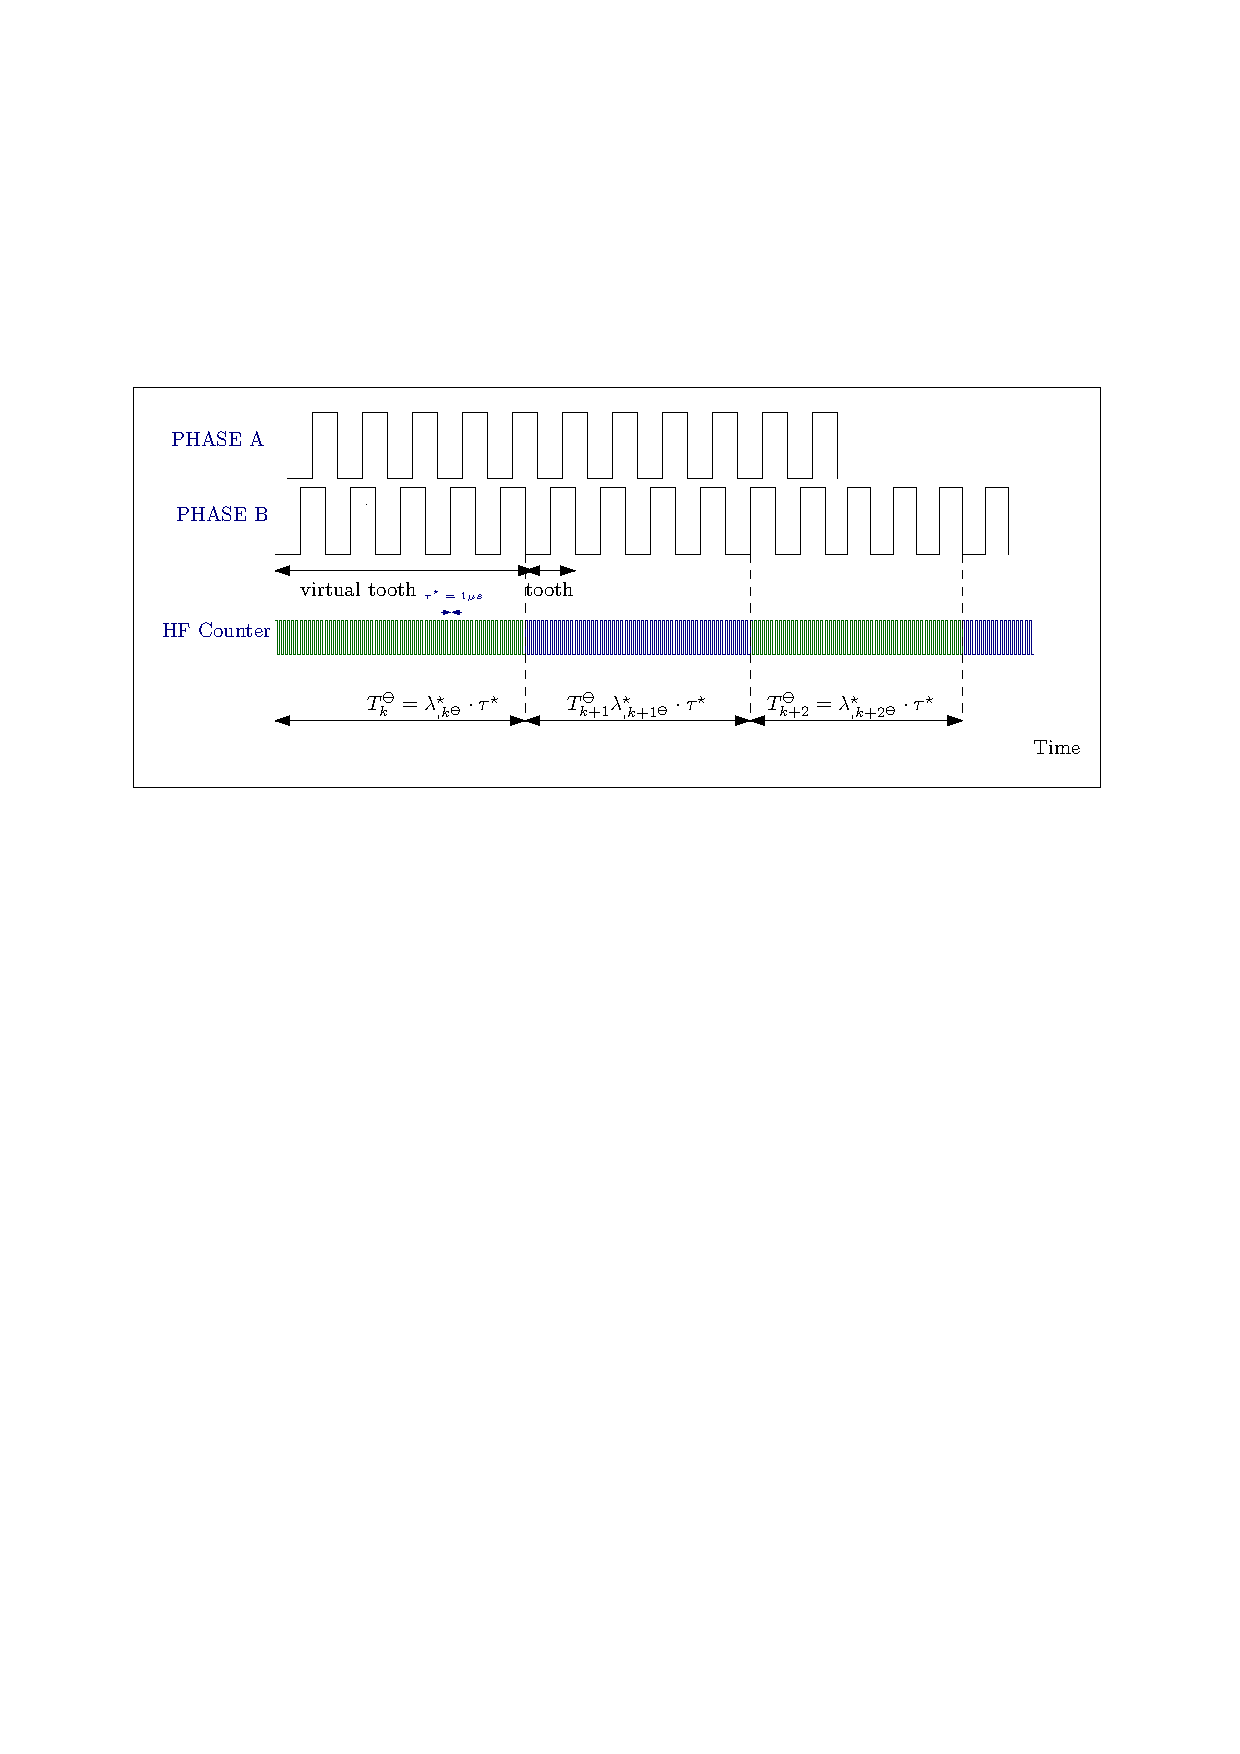
\includegraphics[angle=0,width=.7\textwidth]{period_m.pdf}
}
\caption{\emph{period measure}}
\label {fig:periodenc}
\end{figure}

The implementation of the period measuring method is also
straightforward as it requires a simple timer capture unit,
commonly found inside recent micro-controllers. Specific
hardware subsystems can be considered to overcome digital
timer saturation problems and proper
algorithms are needed to filter out the errors introduced by
sensor nonidealities. The problem of speed
calculation error generated at motor reversion can be easily
solved by the identification of motor direction during time
measurement and correction of the timer value, but best
performance are obtained by means of specific hardware
solutions.




\subsubsection{sensor data}
\paragraph{Delta path (\gls{MMU} cycle path increment)}\footnote {called also delta distance}
The \gls{MMU} processor executes a fetch cycle each $\tau^\circ=50\, \mathrm{m}s$. The samples which are available as raw data are used to calculate the path traveled on the last 50 ms. this is also called Delta-distance or path increment during cycle n.
\begin{equation}
\Delta^\circ_n s = R \Delta^\circ_n \theta = \left(\frac{2\pi R}{N^\ominus} \right) \Delta^\circ_n N^\ominus
\end{equation}
where $\Delta^\circ_n N $ \footnote{Later on where the context is clear we will drop the Delta symbol $\Delta$ and simply write $N^\ominus_{n^\circ}=N^\ominus_{n}$ to indicate the number os samples acquired in the \gls{MMU} cycle n.}  indicates the number of samples cumulated in the \gls{MMU} cycle n. 
\paragraph{current speed}
From the samples $\lambda_{n,k}$ where $n\in[0,\infty] $ is  the index of the \gls{MMU} cycle while $k\in[0,\Delta^\circ_n N^\ominus-1]$ is the index of the samples cumulated in the last cycle at virtual tooth border within the counter array,\footnote{The array has a size NB\_SAMPLES\_MAX, which limits the maximum number of samples, that can be stored in one cycle} the current speed on the cycle n can now be calculated:
\begin{equation}
\varv_{n^\circ} =\frac{\Delta^\circ _n s}{\sum\limits_{k=0}^{\Delta^\circ_n N^\ominus-1}\lambda^\star_{n,k}\tau^\star}  
\end{equation}
\paragraph{smoothed speed}
To avoid small oscillations of the speed due to the eccentricity of the fitted sensor relative to axle of rotation, the speed is smoothed over a full number of wheel revolutions while keeping a delay of 250 ms for the synchronization.
The raw samples of are transferred to a local buffer together with samples of previous cycles.
The sum of the last $N_{\tau^\bullet}$ raw samples (buffered locally) is chosen so that the sum of samples times $\tau^\star$ is immediately less than 500 ms (10 \gls{MMU} cycles) and $N_{\tau^\bullet}$ is a multiple of the number of virtual teeth $N^\ominus$ of the sensor.
\begin{equation}
\Delta^{\bullet}_n N^\ominus=N^\ominus \left\lfloor \frac {\sum\limits_{j=0}^{N^\bullet-1} \Delta^\circ_{n-j}{N^\ominus} }{N^\ominus}\right\rfloor 
\end{equation} 

Where the parenthesis $\left\lfloor \right\rfloor$ indicate integer part (floor). To obtain the raw speed, $\Delta^{\bullet}_n N$ is multiplied by the distance resolution and divided by this sum:
\begin{equation}
\widetilde{\varv}_{n^\bullet}=\frac{ \Delta^{\bullet}_n N^\ominus \left(\frac{2\pi R }{N^\ominus}\right)}{\sum\limits_{j=0}^{N^\bullet-1} \sum\limits_{k=0}^{\Delta^\circ_n N^\ominus-1}\lambda^\star_{n-j,k}\tau^\star}
\end{equation}
\begin{equation}
\widetilde{\varv}_{n^\bullet}=\frac{ \Delta^{\bullet}_n N^\ominus \left(\frac{2\pi R }{N^\ominus}\right)}{ \sum\limits_{\kappa=0}^{\Delta^\bullet_n N^\ominus-1}\lambda^\star_{,\kappa}\tau^\star}
\end{equation}


\begin{figure}[ht!]
\centerline{
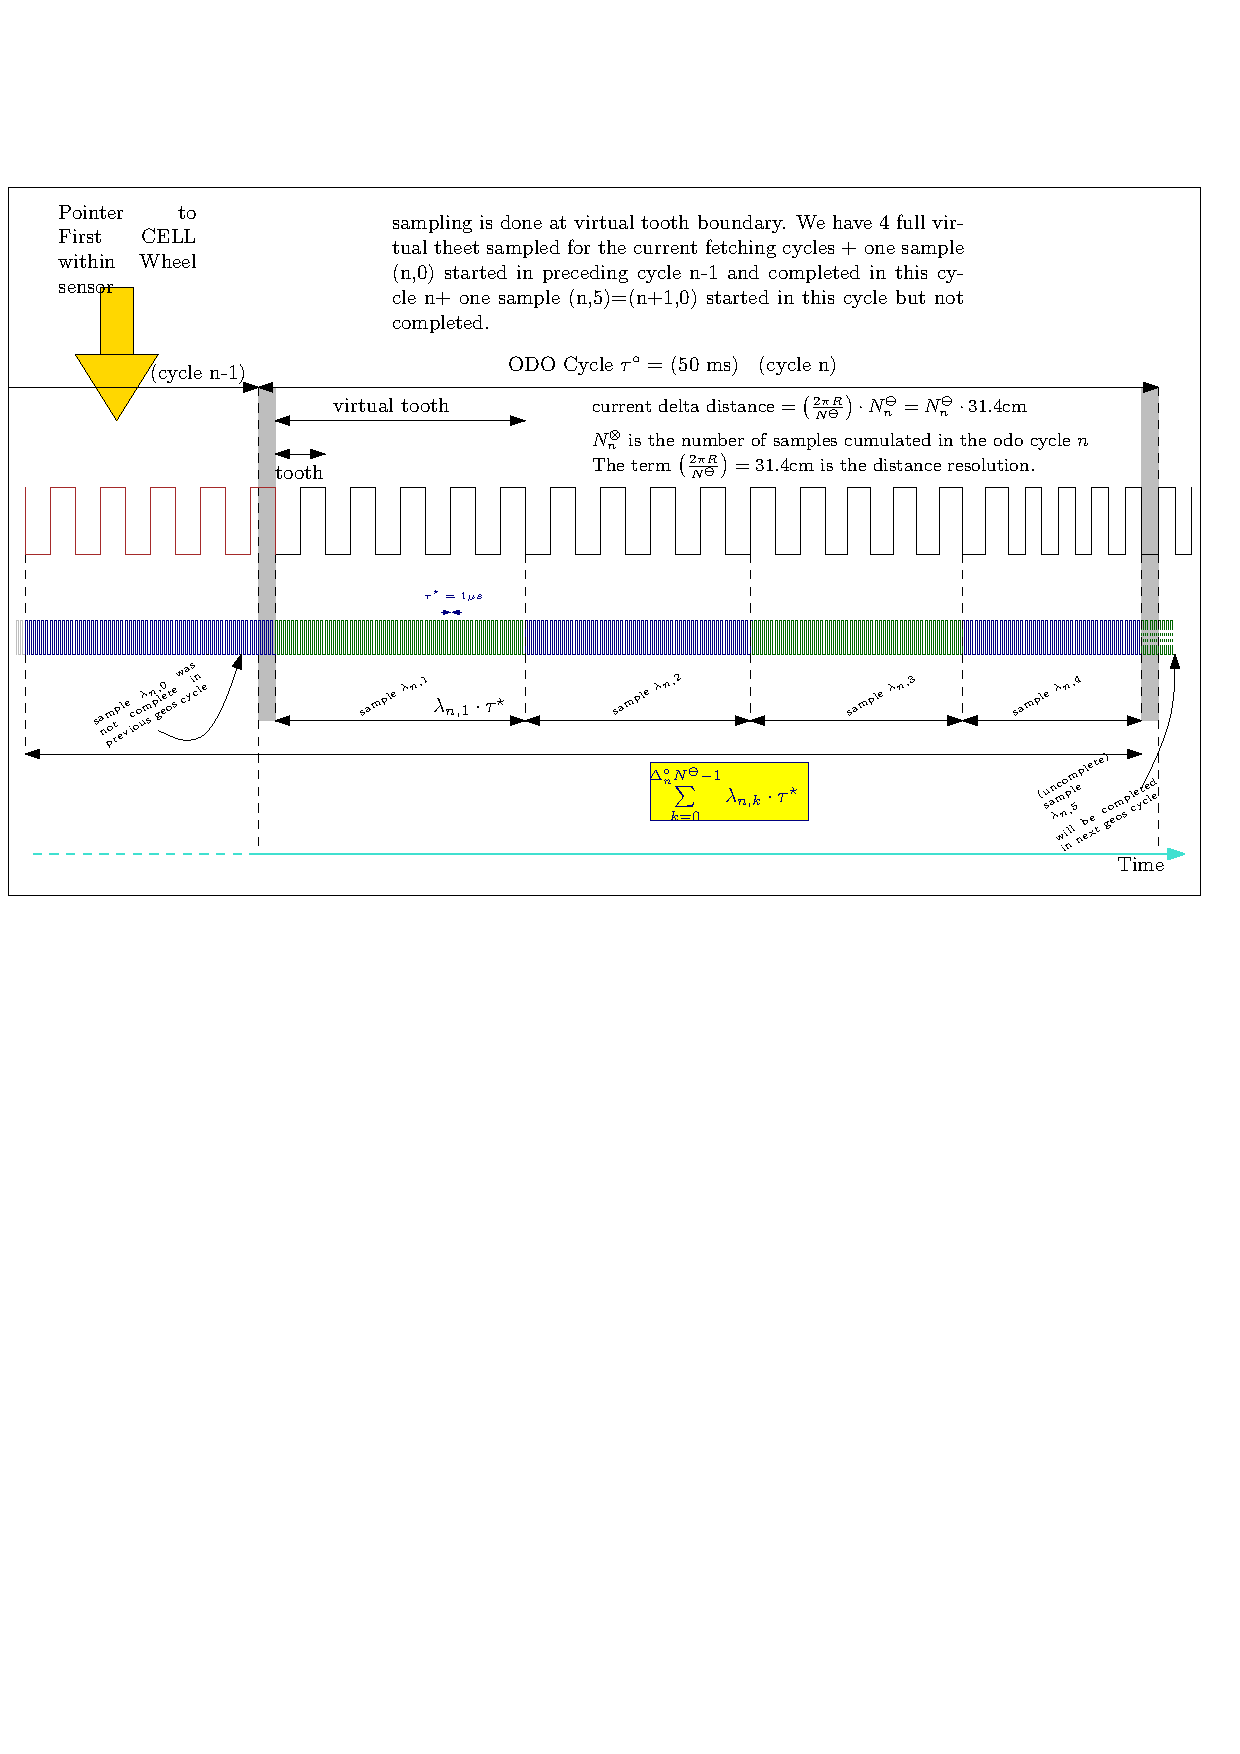
\includegraphics[angle=0,width=1.\textwidth]{teeth_v2.pdf}
}
\caption{\emph{sampling on a \gls{MMU} cycle}}
\label {fig:vteeth_samp}
\end{figure}
\paragraph{moving average over delta path}
The sensors output are to be synchronized every 250 ms. This is achieved by using a moving average on a period of time = (500ms – latency time). The latency time of the sensors has to be less than 250ms. Currently, the used sensors have a negligible latency time and so, the moving average is computed on 500 ms.
The speed estimation is computed using a smoothing mechanism over the speed measurements obtained during the last 500 ms leading to a delay of 250 ms on the speed estimation. The purpose of this mechanism is to smooth the speed measurement and to synchronize at 250 ms the speed estimations between the different
sensors.

The delta-path $(\Delta^\circ_n s )$ will now be averaged using a moving window over the last $N^\bullet$ sampled and stored $\Delta^\circ_{n-j} s$ values (impulses times wheel sensor resolution) acquired in the last 500 ms ($N^\bullet$ cycles = 10 data values).
The expression used for the moving average if we consider also the current value ($j=0$) is given by the formula:
\begin{equation}
\langle \Delta s\rangle^\bullet_n =\frac{1}{N^\bullet}\sum\limits_{j=0}^{N^\bullet-1} \Delta^\circ_{n-j} s 
\end{equation}
which can be updated recurrently at each cycle:
\begin{equation}
\langle \Delta s\rangle^\bullet_{n+1} =\langle \Delta s\rangle^\bullet_{n} +\frac{1}{N^\bullet}\left( \Delta^\circ_{n+1} s -  \Delta^\circ_{n-N+1} s \right)  
\end{equation}
where $N^\bullet=10$ is the size of the sampling buffer and the computation is extended over $N^\bullet$ values including the current data value ($j=0$). The index $n$ on the angular brackets indicates that the sample mean is done on the running buffer containing the data sample trailing the data value acquired at cycle $n$. The index $j$ gives the relative delay of the data point compared to the current data point $n$, while the index $i$ gives the number of the cycle where the data point was acquired, where the number of the fetching cycle has to be considered from the startup of the program, Usually such an index is not available and actual calculations should be made by using the relative index $j$ at each cycle $n$
The life span of a odometry increment is thus equal to 10 cycles. This allows to improve the resolution of the delta-path. The handling of vote mechanism for distance will be than performed voting over the values $\langle \Delta s\rangle^\bullet_{n} $ obtained using the formula above. The corresponding time value should be the one of the center of the averaging window, which is delayed by $j=N/2$ cycles relative to current fetch cycle.  The correct direction has to be associated to the distance increment.

\subsubsection{estimating acceleration from speed measures}

The acceleration can be estimated from the speed data sampled in the current buffer (sample n including current speed measure $\varv_n$) by implementing a linear regression on the sample.
Two possible linear estimators\footnote{\emph{regression} meaning the prevailing of the average over the fluctuations. The concept of \emph{regression to mediocrity}, introduced by Sir Galton reflects the behavior of data when numerous small effects influence and produce fluctuations superposed to systematic behavior. This behavior would certainly not be applicable to a random walk process.} are given by :
\begin{eqnarray}
\hat{\varv}(t_i) &=&\hat{\varv}_n+\hat{a}_n\left(t_i-t_n\right)\label{fig:lin_est1}\\
\hat{\varv}(t_i) &=&\hat{\varv}^{\spadesuit}_n+\hat{a}_n\left(t_i-\langle t \rangle_n\right) \label{fig:lin_est2}
\end{eqnarray}
where the index n indicates the value currently acquired and the associated trailing buffer storing another $N=2M$ sampled data. The total sample will have $N^\bullet$ data points $(\varv_i,t_i)$. The hat symbol will indicate estimated quantities e.g. $\hat{a}_n$ indicates the estimated acceleration over the sample n. There are two parameters to estimate $\hat{\varv}_n$ and $\hat{a}_n$.  The angular brackets indicate the mean value over the sample n obtained by averaging over the $N+1$ data points available at fetching cycle n. For the time value this is the arithmetic mean value (there is no statistical spread over the t variable and the fluctuation on the cycle time $\tau$ is considered negligible). Therefore this value is given only by the buffer size (time window) and can be calculated even without data.
\begin{eqnarray}
\langle t \rangle^\bullet_n &=& \frac{1}{N^\bullet}\sum\limits_{i=n}^{n-N^\bullet+1} t_i \nonumber \\ 
&=& \frac{1}{N^\bullet}\sum\limits_{j=0}^{N^\bullet-1} t_{n-j} \nonumber \\ 
&=& t_{n-N^\bullet/2} \nonumber\\
%&=&  t_{n-M} \nonumber\\
%&=&  t_n-M\tau \nonumber\\
&=&  t_n-\frac{N^\bullet}{2}\tau^\circ
\label{eq:mean_delay}
\end{eqnarray}
\begin{equation}
\boxed{
\langle t \rangle^\bullet_n = t_n-\frac{N^\bullet}{2}\tau
}
\end{equation}
and recurrently:
\begin{equation}
\langle t \rangle^\bullet_{n+1} = \langle t \rangle^\bullet_{n} +\tau^\bullet
\end{equation}

where $M\tau= N/2 \tau$ is the delay of the center of the buffering window (average delay) with respect to the current cycle.
in a similar way for the speed we have:
\begin{equation}
\langle \varv \rangle^\bullet_n=\frac{1}{N^\bullet}\sum\limits_{i=n}^{n-N^\bullet+1} \varv_i =\frac{1}{N^\bullet}\sum\limits_{j=0}^{N^\bullet-1} \varv_{n-j}
\end{equation}
which can be updated recurrently by:
\begin{equation}
\boxed{
\langle \varv \rangle^\bullet_{n+1}=\langle \varv \rangle^\bullet_n +\frac{1}{N^\bullet}\left( \varv_{n+1} - \varv_{n-N^\bullet+1}\right)
}
\end{equation}
\begin{figure}[h!]
\centerline{
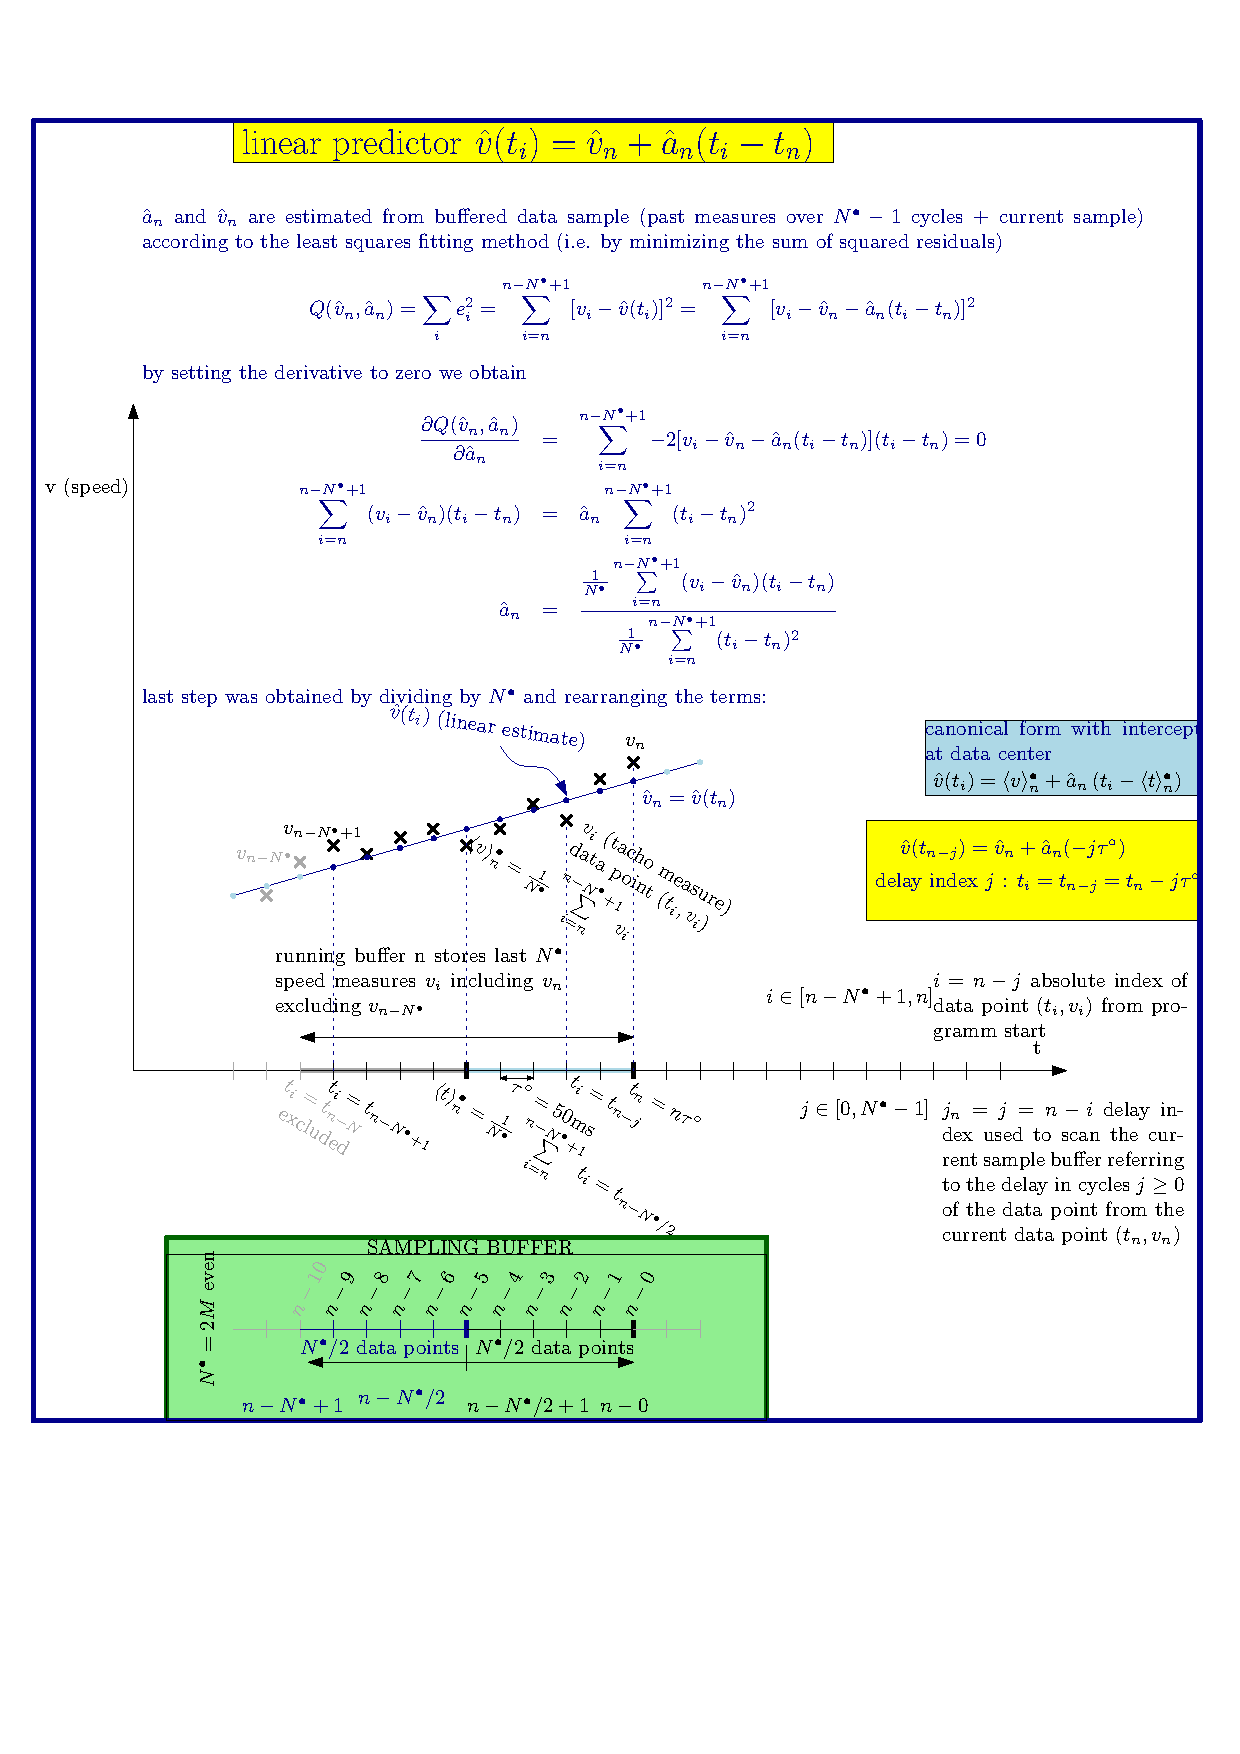
\includegraphics[angle=-0,width=1.\textwidth]{lin_regression_v7.pdf}
}
\caption{\emph{estimate acceleration applying linear regression}}
\label {fig:lregression}
\end{figure}


A way to estimate the parameters of the linear estimator consists in building an error function, aimed to produce a metric by summing up the distance or residual error between acquired data points and estimated data markers \cite{bevington}. This metric will allow to optimize the parameters for the smallest error. One of the most common error function is given by the sum of squared errors, the confidence interval of all data points being assumed identical. This is known as \emph{least square estimation}, and can be applied to a vast spectrum of (not only linear) functions containing parameters e.g. it si applicable for the coefficient estimation of any Fourier sum.

\begin{equation}
Q(\hat{\varv}_n, \hat{a}_n) =\sum\limits_{i=n}^{n-N^\bullet+1} e_i^2=\sum\limits_{i=n}^{n-N^\bullet+1}[ \varv_i-\hat{\varv}(t_i)]^2  =\sum\limits_{i=n}^{n-N^\bullet+1}[\varv_i-\hat{\varv}_n-\hat{a}_n(t_i-t_n)]^2
\end{equation}
We insert one of the selected estimators (\ref{fig:lin_est1}) in the $Q$ function, derive it and put the result to zero to locate the minimum.
\begin{equation}
\frac{\partial Q(\hat{\varv}_n, \hat{a}_n)}{\partial\hat{\varv}_n}=\sum\limits_{i=n}^{n-N^\bullet+1} 2\frac{\partial\hat{\varv}(t_i)}{\partial\hat{\varv}_n}[\varv_i-\hat{\varv}_n-\hat{a}_n(t_i-t_n)]=0
\end{equation}
dividing by $N^\bullet$ this gives:
\begin{eqnarray}
\hat{\varv}_n &=& \frac{1}{N^\bullet} \sum\limits_{i=n}^{n-N^\bullet+1} [\varv_i-\hat{a}_n(t_i-t_n)]\nonumber\\
&=& \langle \varv \rangle^\bullet_n-\hat{a}_n\left [\langle t\rangle^\bullet_n - t_n\right ]
\end{eqnarray}
In a similar way inserting the estimator (\ref{fig:lin_est2}) in the $Q$ function we obtain after derivation:
\begin{eqnarray}
\hat{\varv}^{\star}_n &=& \frac{1}{N^\bullet} \sum\limits_{i=n}^{n-N^\bullet+1} [\varv_i-\hat{a}_n(t_i-\langle t\rangle^\bullet _n)]\nonumber\\
&=& \langle \varv \rangle^\bullet_n
\end{eqnarray}
If we substitute the parameter $ \hat{\varv}_n $ in the original function we obtain in both cases:
\begin{equation}
\boxed{\color{blue}
\hat{\varv}(t_i) =\langle \varv \rangle^\bullet_n + \hat{a}_n\left(t_i-\langle t \rangle^\bullet_n\right)
}
\label{eq:lincan}
\end{equation}

centered on the center of data points sample $(\langle \varv \rangle^\bullet_n,\langle t \rangle^\bullet_n)$.\footnote{With increasing values of $n$ we get $N^\bullet$ different estimates $\hat{\varv}(t_i)$  for the same sample $\varv_i$, as the averaging window is moving forward in time.}
This is a 
%\colorbox{yellow}
{canonical form} for the linear predictor reflects the fact that the linear estimation function always includes
%\colorbox{yellow}
{the center} of the data sample. The second parameter $\hat{a}_n$ being the inclination of the line pivoting about the data sample center. 
The estimated value for the last sample is given by adding the estimated acceleration over the half window period to the window center velocity value $\varv(\langle t\rangle_n)=\langle \varv\rangle_n $
\begin{equation}
\hat{\varv}(t_n) =\langle \varv \rangle^\bullet_n + \hat{a}_n\frac{N^\bullet}{2} \tau^\circ
\end{equation}

The error function becomes:
\begin{equation}
\boxed{
Q(\hat{\varv}_n, \hat{a}_n) = \sum\limits_{i=n}^{n-N^\bullet+1}[ \varv_i-\langle \varv \rangle^\bullet_n - \hat{a}_n\left(t_i-\langle t \rangle^\bullet_n\right)]^2
}
\end{equation}
We use now this expression to get the estimation of the second parameter $\hat{a}_n$
\begin{equation}
\frac{\partial Q(\hat{\varv}_n, \hat{a}_n)}{\partial\hat{a}_n}=\sum\limits_{i=n}^{n-N^\bullet+1} 2\frac{\partial\hat{\varv}(t_i)}{\partial\hat{a}_n}[\varv_i-\langle \varv \rangle^\bullet_n -\hat{a}_n(t_i-\langle t\rangle^\bullet_n)]=0
\end{equation}
dividing by $N^\bullet$ and reordering we get
\begin{equation}
\frac{1}{N^\bullet}\sum\limits_{i=n}^{n-N^\bullet+1} [\varv_i-\langle \varv \rangle^\bullet_n -\hat{a}_n(t_i-\langle t\rangle^\bullet_n)](t_i-\langle t\rangle^\bullet_n)=0
\end{equation}

\begin{equation}
\boxed{
\hat{a}_n=\frac{\frac {1}{N^\bullet}\sum\limits_{i=n}^{n-N^\bullet+1}(\varv_i - \langle \varv \rangle^\bullet_n)(t_i-\langle t\rangle^\bullet_n)}{\frac {1}{N^\bullet} \sum\limits_{i=n}^{n-N^\bullet+1}(t_i- \langle t\rangle^\bullet_n)^2}=\frac{\langle \varv \cdot t\rangle^\bullet_n - \langle \varv \rangle^\bullet_n \langle t\rangle^\bullet_n}{\langle t^2\rangle^\bullet_n- \langle t \rangle^{\bullet 2}_n}
}
\label{eq:aest}
\end{equation}

the expression for $\langle t\rangle_n $ was already given in \ref{eq:mean_delay}. We still  need the expression for $\langle t^2\rangle_n$. Both $\langle t^2\rangle^\bullet_n$ and $\langle (t - \langle t^2\rangle^\bullet_n)^2\rangle^\bullet_n$ are characterized only by the buffer size and are data independent, while $\langle \varv \cdot t\rangle^\bullet_n$ and $\langle \varv \rangle^\bullet_n$ have to be evaluated from data.
\begin{eqnarray}
\frac {1}{N^\bullet}\sum\limits_{i=n}^{n-N^\bullet+1} (t_i - \langle t\rangle^\bullet_n)^2 &=&
\langle t^2\rangle^\bullet_n- \langle t\rangle^{\bullet 2}_n \nonumber\\
&=& \langle( t - \langle t\rangle^\bullet_n)^2\rangle^\bullet_n
\end{eqnarray}
Recalling that $ \langle t\rangle^\bullet_n = t_n-\frac{N^\bullet}{2}\tau^\circ$ we get:
\begin{eqnarray}
\frac {1}{N^\bullet}\sum\limits_{i=n}^{n-N^\bullet+1} \tau^{\circ 2} \left (i - n + \frac{N^\bullet}{2}\right )^2 &=&\nonumber\\
\frac { \tau^{\circ 2} }{N^\bullet}\sum\limits_{j=0}^{N^\bullet-1}(\frac{N^\bullet}{2}-j)^2 &=& \tau^{\circ 2} \frac{(N^\bullet-1)(N^\bullet+1)}{12}
\end{eqnarray}
where we have changed the index $i-n=-j$
\begin{equation}
\boxed{\color{blue}
\frac {1}{N^\bullet}\sum\limits_{i=n}^{n-N^\bullet+1} \left (t_i - \langle t\rangle^\bullet _n\right)^2=\tau^{\circ 2} \frac{(N^\bullet-1)(N^\bullet+1)}{12}
}
\end{equation}


In a similar fashion :
\begin{eqnarray}
\frac {1}{N^\bullet}\sum\limits_{i=n}^{n-N^\bullet+1} (t_i - \langle t\rangle^\bullet_n) &=&
\langle t - \langle t\rangle^\bullet_n\rangle^\bullet_n \nonumber\\
&=& \langle t \rangle^\bullet_n - \langle t\rangle^\bullet_n \nonumber\\ &=& 0
\end{eqnarray}

\clearpage
and so finally the equation \ref{eq:aest} becomes:  
\marginpar{\footnotesize $\Leftarrow $ by using: 
$$
\langle \varv \rangle_n\sum\limits_{i=n}^{n-N}(t_i-\langle t\rangle_n)=0
$$
}
\begin{eqnarray}
\hat{a}_n &=& \frac{\frac {1}{N^\bullet}\sum\limits_{i=n}^{n-N^\bullet+1}(\varv_i - \langle \varv \rangle^\bullet_n)(t_i-\langle t\rangle^\bullet_n)}{\frac {1}{N^\bullet} \sum\limits_{i=n}^{n-N^\bullet+1}(t_i- \langle t\rangle^\bullet_n)^2}\nonumber\\
&=& \frac{\frac {1}{N^\bullet}\sum\limits_{i=n}^{n-N^\bullet+1} \varv_i (t_i-\langle t\rangle^\bullet_n)}{\frac {\tau^{\circ 2} (N^\bullet-1)(N^\bullet+1)}{12} }\nonumber\\
&=& \frac{\frac {1}{N^\bullet}\sum\limits_{i=n}^{n-N^\bullet+1} \varv_i t_i -\frac {\langle t\rangle^\bullet_n }{N^\bullet}\sum\limits_{i=n}^{n-N^\bullet+1}\varv_i}{\frac {\tau^{\circ 2} (N^\bullet-1)(N^\bullet+1)}{12} }\nonumber\\
&=& \frac{\frac {1}{N^\bullet}\sum\limits_{j=0}^{N^\bullet-1} \varv_{n-j} t_{n-j} -\langle t\rangle^\bullet_n \langle \varv \rangle^\bullet_n}{\frac {\tau^{\circ 2} (N^\bullet-1)(N^\bullet+1)}{12} }\nonumber\\
&=& \frac{\frac {1}{N^\bullet}\sum\limits_{j=0}^{N^\bullet-1} \varv_{n-j} (t_n- j\tau^\circ) -\langle t\rangle^\bullet_n \langle \varv \rangle^\bullet_n}{\frac {\tau^{\circ 2} (N^\bullet-1)(N^\bullet+1)}{12} }\nonumber\\
&=& \frac{\frac {t_n}{N^\bullet}\sum\limits_{j=0}^{N^\bullet-1} \varv_{n-j} -\frac{\tau^\circ}{N^\bullet}\sum\limits_{j=0}^{N^\bullet-1} j\cdot \varv_{n-j} -\langle t\rangle^\bullet_n \langle \varv \rangle^\bullet_n}{\frac {\tau^{\circ 2} (N^\bullet-1)(N^\bullet+1)}{12} }\nonumber\\
&=& \frac{\langle \varv \rangle^\bullet_n (t_n-\langle t\rangle^\bullet_n ) -\frac{\tau^\circ }{N^\bullet}\sum\limits_{j=0}^{N^\bullet-1} j\cdot \varv_{n-j}}{\frac {\tau^{\circ 2} (N^\bullet-1)(N^\bullet+1)}{12} }\nonumber\\
&=& \frac{\langle \varv \rangle^\bullet_n \frac{\tau^\circ N^\bullet}{2} -\frac{\tau^\circ}{N^\bullet}\sum\limits_{j=0}^{N^\bullet-1} j\cdot \varv_{n-j}}{\frac {\tau^{\circ 2} (N^\bullet-1)(N^\bullet+1)}{12} }
\end{eqnarray}

\begin{equation}
\boxed{\color{blue}
\hat{a}_n= \left( \langle \varv \rangle^\bullet_n \frac{\tau^\circ N^\bullet}{2} -\frac{\tau^\circ}{N^\bullet}\sum\limits_{j=0}^{N^\bullet-1} j\cdot \varv_{n-j}\right) \frac {12}{\tau^{\circ 2} (N^\bullet-1)(N^\bullet+1)} 
}
\label{eq:aestls}
\end{equation}
which can be evaluated recurrently:
\begin{equation}
\boxed{\color{blue}
\hat{a}_{n+1}= \hat{a}_{n}+ \frac{6}{\tau^\circ }\frac{(N^\bullet-1)\varv_{n+1}-2N^\bullet\langle \varv\rangle^\bullet_n+(N^\bullet+1)\varv_{n-N^\bullet}}{ (N^\bullet-1)N^\bullet(N^\bullet+1)} 
}
\end{equation}

To obtain this relation simply substitute $n\rightarrow n+1$ in the definition \ref{eq:aestls}
\begin{equation}
\begin{array}{ll}
{\displaystyle \hat{a}_{n+1}} &{\displaystyle = \left( \langle \varv \rangle^\bullet_{n+1} \frac{N^\bullet}{2} -\frac{1}{N^\bullet}\sum\limits_{j=0}^{N^\bullet-1} j\cdot \varv_{n+1-j}\right) \frac {12}{\tau^\circ (N^\bullet-1)(N^\bullet+1)}} \\ 
&{\displaystyle = \left(\left( \langle \varv \rangle^\bullet_{n}+\frac{ \varv_{n+1}-\varv_{n-N^\bullet+1}}{N^\bullet} \right)\frac{N^\bullet}{2} -\frac{1}{N^\bullet}\sum\limits_{j=0}^{N^\bullet-1} j\cdot \varv_{n-(j-1)}\right) \frac {12}{\tau^\circ (N^\bullet-1)(N^\bullet+1)}} \\
&{\displaystyle = \left(\left( \langle \varv \rangle^\bullet_{n}+\frac{ \varv_{n+1}-\varv_{n-N^\bullet+1}}{N^\bullet} \right)\frac{N^\bullet}{2} -\frac{1}{N^\bullet}\sum\limits_{j=-1}^{N^\bullet-2} (j+1)\cdot \varv_{n-j}\right) \frac {12}{\tau^\circ (N^\bullet-1)(N^\bullet+1)}} \\
&{\displaystyle = \left(\left( \langle \varv \rangle^\bullet_{n}+\frac{ \varv_{n+1}-\varv_{n-N^\bullet+1}}{N^\bullet} \right)\frac{N^\bullet}{2} -\frac{\sum\limits_{j=0}^{N^\bullet-1} j\cdot \varv_{n-j}}{N^\bullet}+\varv_{n-N^\bullet+1}-\langle \varv\rangle^\bullet_n \right) \frac {12}{\tau^\circ (N^\bullet-1)(N^\bullet+1)}} \\
&{\displaystyle = \hat{a}_n+ \left( \frac{ \varv_{n+1}-\varv_{n-N^\bullet+1}}{N^\bullet} \frac{N^\bullet}{2} +\varv_{n-N^\bullet+1}-\langle \varv\rangle^\bullet_n \right) \frac {12}{\tau^\circ (N^\bullet-1)(N^\bullet+1)}} \\
&{\displaystyle = \hat{a}_n + \left( \frac{ \frac{N^\bullet}{2}\varv_{n+1}+\left(\frac{N^\bullet}{2}+1\right)\varv_{n-N^\bullet+1}-(N^\bullet)\langle \varv\rangle^\bullet_n}{N^\bullet} \right) \frac {12}{\tau^\circ (N^\bullet-1)(N^\bullet+1)}} \\
\end{array}
\end{equation}



\subsubsection{Goodness of fit}
If the deviations from the mean follow a Gaussian statistics, the probability of making any one observation $v_i$ at time $t_i$ is given by:
\begin{equation}
P(\varv_i)=\frac{1}{\sigma_i\sqrt{2\pi}}\exp\left (-\frac{\left [\varv_i-\mu(t_i)\right]^2}{2\sigma_i^2}\right)
\approx\frac{1}{\sigma_i\sqrt{2\pi}}\exp\left (-\frac{\left [\varv_i-\hat{\varv}(t_i)\right]^2}{2\sigma_i^2}\right)
\end{equation}
where we use the linear estimate $v(t_i)$ as estimate of the mean value $\mu(t_i)$ of the Gaussian being the value of velocity if measured at time $t_i$ with an hypothetical error-free device.
The total probability of obtaining a set of $N+1$ measurements,$ \{t_i ,\varv_i \}$, is
equal to the product of the probabilities for each data point:
\begin{equation}
\prod_{i=N-n}^nP(\varv_i)\approx\prod_{i=N-n}^n\left \{ \frac{1}{\sigma_i\sqrt{2\pi}}\exp\left (-\frac{\left [\varv_i-\hat{\varv}(t_i)\right]^2}{2\sigma_i^2}\right)\right\}
\end{equation}
\begin{figure}[h!]
\centerline{
%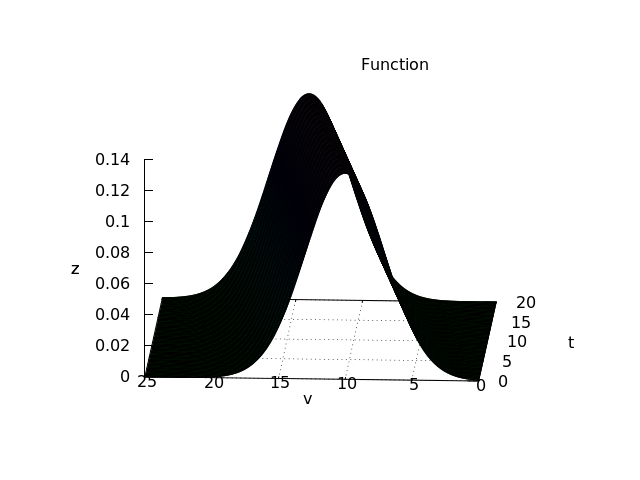
\includegraphics[angle=-0,width=.3\textwidth]{parent_pdf_d.png}
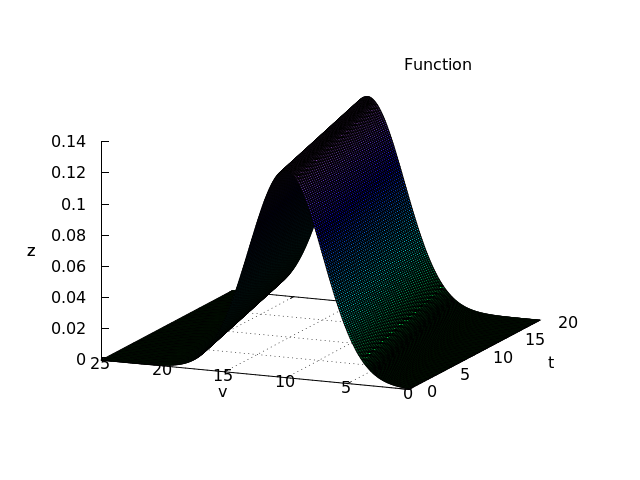
\includegraphics[angle=-0,width=.5\textwidth]{parent_pdf_a.png}
%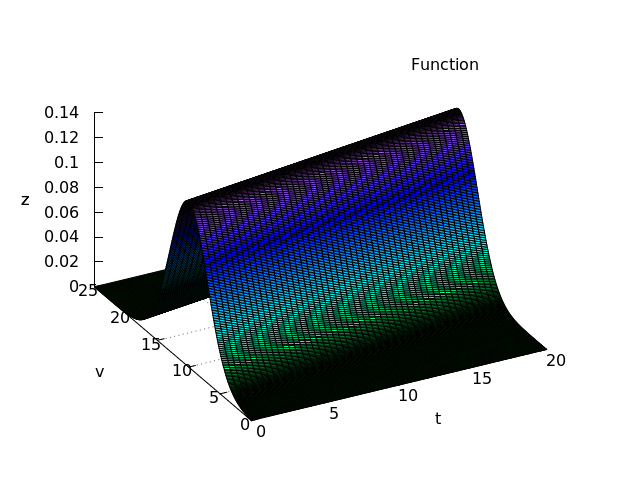
\includegraphics[angle=-0,width=.3\textwidth]{parent_pdf_b.png}
}
\caption{\emph{Gaussian family with "drifting" mean and constant variance}}
\label {fig:parent_pdf}
\end{figure}




\noindent
%%%%%%%%%%%%%%%
%%% INPUT:
%\begin{minipage}[t]{8ex}{\color{red}\bf
%\begin{verbatim}
%(%i36) 
%\end{verbatim}
%}
%\end{minipage}
%\begin{minipage}[t]{\textwidth}{\color{blue}
%\begin{verbatim}
%plot3d(1/(3*sqrt(2*%pi))*exp(-(v-10-0.2*t)^2/18), 
% [t,0,20], [v,0,25], [plot_format,gnuplot],
% [grid,50,350],
% [gnuplot_pm3d,true],
% [gnuplot_preamble, "set hidden3d"])$
%\end{verbatim}
%}
%\end{minipage}


Maximizing the probability is equivalent to minimize the sum in the exponential term of $ P (\{\varv,t\}) $ , specifically the sum of the deviations weighted by $\sigma^2_i$,
\begin{equation}
\sum\limits_{i=N-n}^n\frac{e_i^2}{2\sigma^2_i}=
\sum\limits_{i=N-n}^n\frac{\left [\varv_i-\hat{\varv}(t_i)\right]^2}{2\sigma^2_i}
\end{equation}
\footnote{ In case of variable variance $\sigma_i$ the expression to be maximized is
\begin{equation}
\prod\limits_{i=N-n}^n\frac{1}{\sqrt{2\pi}} exp\left( -\frac{\left [\varv_i-\hat{\varv}(t_i)\right]^2}{2\sigma^2_i}- \log\sigma_i\right)
\end{equation}
and therefore the exponent to be minimized is:
\begin{equation}
\sum\limits_{i=N-n}^n\left( \frac{\left [\varv_i-\hat{\varv}(t_i)\right]^2}{2\sigma^2_i}+ \log\sigma_i\right)
\end{equation}

But as we parametrize only the model estimating the mean value of $\hat{\varv(t_i)}$ the term $\log\sigma_i$ is a constant and can be ignored. The model predicts only the mean value and tries not to guess the variance interval.}
In the special case where all the $\sigma_i$ are identical we are we are led back to the least squares principle.
The chi-square statistic is defined by following sum where we replace the absolute index $i$ with the relative index $j$  $(i=n-j)$:
\begin{equation}
\boxed{
\chi^2=\sum\limits_{j=0}^{N}\frac{e_{n-j}^2}{\sigma^2_{n-j}}=
\sum\limits_{j=0}^{N}\frac{\left [\varv_{n-j}-\hat{\varv}(t_{n-j})\right]^2}{\sigma^2_{n-j}}
}
\end{equation}

If the terms of the sum are of the order of $\approx 1$ we get that $\chi$ increases with the number of observations $N+1$. The method of least squares is built on the hypothesis that the optimum
description of a set of data is one which minimizes the weighted sum of squares of deviations, $e_i$, between the data, $\varv_i$ , and the fitting function $\hat{\varv}(t_i)$.

The sum of squares of deviations is characterized by the “estimated variance of the fit”, $s^2$ , which is an estimate of the variance of the parent distribution, $\sigma^2$.
\begin{eqnarray}
s^2=\frac{1}{N+1}\sum\limits_{j=0}^{N} (\varv_{n-j}-\hat{\varv}(t_{n-j}))^2\nonumber\\
\sigma^2=\lim\limits_{N\to\infty}\frac{1}{N+1}\sum\limits_{j=0}^{N} (\varv_{n-j}-\mu(t_{n-j}))^2
\end{eqnarray}

The ratio of $s^2 /\sigma^2$ can be estimated by $\chi^2 / \nu$, where %\colorbox{yellow}
{ $ \nu  = N +1 - p $} is called degree of freedom, $N+1$ is the number of observations and $p$ is the number of fitting parameters. The expression $\chi^2 / \nu$ is called the 
%\colorbox{yellow}
{reduced chi-square} statistic.
For $p=2$ we get $\nu=N-1$ :
\begin{equation}
\boxed{
\frac{\chi^2}{\nu}=\frac{1}{N-1}\sum\limits_{j=0}^{N}\frac{\left [\varv_{n-j}-\hat{\varv}(t_{n-j})\right]^2}{\sigma^2_{n-j}}
}
\end{equation}

If the fitting function $\hat{\varv}(t_{n-j})$ accurately predicts the means $\mu(t_{n-j})$\footnote{the velocity at time $t_{n-j}$ measured with a much better device, having a much smaller error} of the parent distribution, then the estimated variance, $s^2$ , should agree well with the variance of the parent distribution, $\sigma^2$ , and their ratio should be close to one.
This explains the origin of the rule of thumb for chi-square fitting that states that a “good fit” is achieved when the reduced chi-square equals one.
The Chi-Square $(\chi^2 )$ distribution function gives the probability distribution for any quantity which is the sum of the squares of independent, normally-distributed variables with unit variance. In is used in the method of maximum likelihood for testing the functional relationship between measured quantities.
\begin{equation}
\boxed{
p(\chi^2,\nu)=\frac{1}{2^{\frac{\nu}{2}}\Gamma(\frac{\nu}{2})}\left(\chi^2\right)^{\frac{\nu-2}{2}}\exp\left[-\frac{\chi^2}{2}\right]
}
\end{equation}

Resuming the least squares method gives a general principle to obtain a fitting between a N-diemnsional vector $(v_i)$ of measured data with an N-dimensional vector produced by a model using 2 or more parameters. The parameters are used to assemble a linear combination of the base functions of the model space, they can be polynomial, periodic function or ...in the simplest case two parameters are used to produce a straight line. (linearity of the model space and linearity of function). There is no reference to any distribution or likelihood until here simply a minimum distance principle in the N-dimensional data space between observed vector $(\varv_0,\varv_1,\varv_2 \ldots \varv_N)$ and the synthetic vector $(\hat{\varv}(t_0),\hat{\varv}(t_1),\hat{\varv}(t_2),\ldots \hat{\varv}(t_N) )$
It emerges that if the data vector can be assumed to be subjected to an Gaussian error with constant variance, the least squares principle satisfies also a maximum likelihood principle. And the vector distance normalized by the factor $\sigma$ obeys a $\chi^2$ probability distribution function, which can be used to evaluate the  estimate the confidence interval. We define as above the error between the sampled speed and the speed value estimated with the linear regression:
\begin{equation}
e_i = \varv_i-\hat{\varv}(t_i) = \varv_i-\langle \varv \rangle_n + \hat{a}_n\left(t_i-\langle t \rangle_n\right)
\end{equation}
(see above \ref{eq:lincan}). and squaring:
\begin{equation}
e^2_i=(\varv_i-\langle \varv \rangle_n)^2+ 2(\varv_i-\langle \varv \rangle_n )(\hat{a}_n\left(t_i-\langle t \rangle_n\right)) + \hat{a}_n^2\left(t_i-\langle t \rangle_n\right)^2
\end{equation}

\begin{eqnarray}
\frac{1}{N+1}\sum\limits_{j=0}^{N}e^2_{n-j}&=&\frac{1}{N+1}\sum\limits_{j=0}^{N}(\varv_{n-j}-\langle \varv \rangle_n)^2\nonumber \\
&+& \frac{2}{N+1}\sum\limits_{j=0}^{N}(\varv_{n-j}-\langle \varv \rangle_n )(\hat{a}_n\left(t_{n-j}-\langle t \rangle_n\right))\nonumber \\ 
&+&\frac{1}{N+1}\sum\limits_{j=0}^{N}\hat{a}_n^2\left(t_{n-j}-\langle t \rangle_n\right)^2
\end{eqnarray}
\begin{eqnarray}
\frac{1}{N+1}\sum\limits_{j=0}^{N}e^2_{n-j}&=&\langle (v-\langle \varv \rangle_n)^2\rangle_n \nonumber \\
&+& 2\hat{a}_n\langle \left(v-\langle \varv \rangle_n \right)\cdot \left(t-\langle t \rangle_n\right)\rangle_n \nonumber \\ 
&+&\hat{a}_n^2\langle \left(t-\langle t \rangle_n\right)^2\rangle_n
\end{eqnarray}
  
the chi square indicates the variance of the error
\begin{equation}
\chi^2_{red}(e)=\frac{1}{N-1}\sum\limits_{j=0}^{N}e^2_{n-j}
\end{equation}

\subsection{measuring accelerations }
\begin{figure}[!ht]
%\boxed{
\centerline{
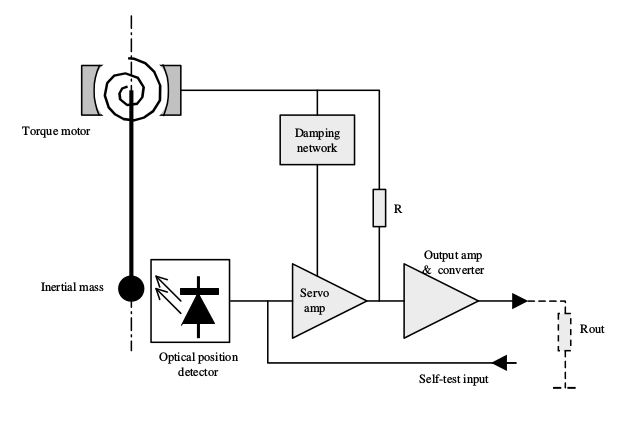
\includegraphics[angle=-0,width=.5\textwidth]{sensor.png}
}
%}
\caption{\emph{sketch of accelerometer}}
\label{fig:sensor}
\end{figure}
The accelerometer is intended to measure the acceleration along the train path (in tangent direction to the train path). The device  is calibrated in defined conditions when the train is in horizontal position and it is set up to have an equal elongation range for acceleration and for deceleration on a rectilinear route. 

It should be noticed, that if the train is moving freely downhill the acceleration measured by this device will be null, according to equivalence principle. On the other side if the train stands still with applied brake on a track with gradient the device will measure a deceleration given by $g\cdot\sin\iota\approx g\cdot\iota $, which will be of the order of $0.x \,\, m/s^2$ for typical gradient values. This effect corresponds to the braking force applied to the train to hold it still. 

This force is not producing work in the rest frame because there is no displacement and it is not producing work in any other reference because in the still stand the braking force compensates exactly the gradient force. 

If the train is accelerating by effect of traction force the measured value shall correspond to the (averaged) acceleration due to the traction. 
In other words the measured acceleration is only the contribution due to applied traction or brake but not the contribution from the gradient. In order to know the tangential acceleration component due to gradient we should (at least in theory) measure the acceleration component normal to the rail $g\cdot\cos\iota \approx g\cdot \left(1-\frac{1}{2}\iota^2 \right) $. 

The loss of weight would be only of the second order in the gradient and indicate a corresponding downhill acceleration or an uphill deceleration.
